\documentclass[10pt,twocolumn,letterpaper]{article}

\usepackage{iccv}
\usepackage{times}
\usepackage{epsfig}
\usepackage{graphicx}
\usepackage{amsmath}
\usepackage{amssymb}
\usepackage{booktabs}
\usepackage{todonotes}
\usepackage{enumitem}
\usepackage{pifont}
\usepackage{algorithm}
\usepackage{algpseudocode}
\usepackage{multirow}
\usepackage{blindtext}
\usepackage{subcaption}
\usepackage{tabularray}
\usepackage{array}
\usepackage{bbding}
\usepackage{pifont}
\usepackage[numbers]{natbib}
\algnewcommand\algorithmicforeach{\textbf{for each}}
\algdef{S}[FOR]{ForEach}[1]{\algorithmicforeach\ #1\ \algorithmicdo}
\usepackage{color}

\newcommand{\cc}{\color[rgb]{0,0.6,0.3}\checkmark}
\newcommand{\xx}{\color[rgb]{0.6,0,0}{\ding{55}}}
\newcommand{\cmark}{\ding{51}}
\newcommand{\xmark}{\ding{55}}

% \newcommand\todoShibo[1]{\todo[fancyline,author=Shibo,color=red]{#1}}
% \newcommand\todoJiahe[1]{\todo[fancyline,author=Jiahe,color=green]{#1}}
% \newcommand\todoDaman[1]{\todo[fancyline,author=Daman,color=orange]{#1}}
% \newcommand\todoRushan[1]{\todo[fancyline,author=Rushan,color=blue]{#1}}
% \newcommand\todoSean[1]{\todo[fancyline,author=Sean,color=yellow]{#1}}
% \newcommand\todoSourojit[1]{\todo[fancyline,author=Sourojit,color=black]{#1}}
% \newcommand\todoJay[1]{\todo[fancyline,author=Jay,color=cyan]{#1}}
% \newcommand\todoChuck[1]{\todo[fancyline,author=Chuck,color=purple]{#1}}
% \newcommand\todoIan[1]{\todo[fancyline,author=Ian,color=pink]{#1}}


\usepackage{cancel}


% Include other packages here, before hyperref.

% If you comment hyperref and then uncomment it, you should delete
% egpaper.aux before re-running latex.  (Or just hit 'q' on the first latex
% run, let it finish, and you should be clear).
\usepackage[breaklinks=true,bookmarks=false, hidelinks]{hyperref}


\usepackage[capitalize]{cleveref}
\crefname{section}{Sec.}{Secs.}
\Crefname{section}{Section}{Sections}
\Crefname{table}{Table}{Tables}
\crefname{table}{Tab.}{Tabs.}
\iccvfinalcopy % *** Uncomment this line for the final submission

\def\iccvPaperID{****} % *** Enter the ICCV Paper ID here
\def\httilde{\mbox{\tt\raisebox{-.5ex}{\symbol{126}}}}

% Pages are numbered in submission mode, and unnumbered in camera-ready
\ificcvfinal\pagestyle{empty}\fi



%%%%%%%%% TITLE
\title{SubT-MRS: A Subterranean, Multi-Robot, Multi-Spectral and\\Multi-Degraded Dataset for Robust SLAM}


\author{\large Shibo Zhao \thanks{Corresponding author: shiboz.andrew.cmu.edu.}  \textsuperscript{1} \quad Damanpreet Singh \textsuperscript{1} \quad Haoxiang Sun\textsuperscript{1}  \quad Rushan Jiang\textsuperscript{1} \quad Tianhao Wu\textsuperscript{1} \\  \quad Yuanjun Gao  \textsuperscript{1} \quad Jay Karhade  \textsuperscript{1} \quad Ian Higgins  \textsuperscript{1} \quad Warren Whittaker
\textsuperscript{1}  \quad Lucas Nogueira   
\textsuperscript{1} \\
\quad Tingting Da \textsuperscript{1}  \quad Mansi Sarawata  
\textsuperscript{1} \quad Can Xu  \textsuperscript{1} \quad Jiahe Xu \quad He Yao  \textsuperscript{1}  \\  
\quad Sourojit Saha  \textsuperscript{1} 
\quad Yuheng Qiu  \textsuperscript{1} \quad Wenshan Wang  \textsuperscript{1}   
\quad Chen Wang  \textsuperscript{1} \quad Sebastian Scherer 
\textsuperscript{1} \vspace{1.5 mm}\\
	{\normalsize \textsuperscript{1}Carnegie Mellon University \quad }  
    % {\tt\footnotesize \{gyd2011@mail., kychern@mail., juyong@\}ustc.edu.cn} \\
    % {\tt\footnotesize \{liangsen\_2014@, bao@cad.\}zju.edu.cn} \hspace{1 mm} 
    % {\tt\footnotesize liuyongjin@tsinghua.edu.cn} 
    }



% \author{Shibo Zhao\\
% Robotics Institute\\
% {\tt\small shiboz@andrew.cmu.edu}
% % For a paper whose authors are at the same institution,
% % omit the following lines up until the closing ``}''.
% % Additional authors and addresses can be added with ``\and'',
% % just like the second author.
% % To save space, use either the email address or home page, not both
% \and
% Second Author\\
% Institution2\\
% First line of institution2 address\\
% {\tt\small secondauthor@i2.org}
% }

% \author{Shibo Zhao\\
% \and
% Haoxiang Sun\\
% \and
% Rushan Jiang\\
% \and
% Damanpreet Singh,
% \and 
% YuanJun Gao \\
% \and
% Tianhao Wu \\
% \and 
% Jay Karhade\\
% \and
% Ian Higgins\\
% \and
% Warren Whittaker\\
% \and
% Jiahe Xu\\
% \and
% Sourojit Saha\\
% \and
% Chen Wang\\
% \and
% Sebastian Scherer\\
% }

% \listoftodos

% \vfill\null

% \textbf{GLOBAL TO-DOs:}
%  \begin{itemize}
%      \item Sean : Replace old pictures with new ones (groundtruth, subt, etc)
%      \item Jay : Polish/proof-read descriptions of pictures/charts  (Use different robots from different projects and need clarify contact Shibo for detail)
%      \item Jay : Double-check the figure/table index and their placement 
%      \item Sourojit : Grammar Checking (using tools like grammarly)
%      \item Daman,Shibo : Check consistency and language between paragraphs
%      \item Shibo : Paper format change to ICCV & length control (8 page excluding references)
%  \end{itemize}



% \maketitle
% % Remove page # from the first page of camera-ready.
\setlength {\marginparwidth }{2cm} 
\ificcvfinal\thispagestyle{empty}\fi
\begin{document}
\twocolumn[{% 
    \renewcommand\twocolumn[1][]{#1}% 
    \maketitle 
    \begin{center} 
    \centering 
    \includegraphics[width=0.9\linewidth]{figure/groundtruth_show_6.png} \captionof{figure}{Ground truth dense, high-quality reconstruction map and Ground truth trajectory generation } 
    \label{fig:ground_truth}
    \end{center}% 
}]


%%%%%%%%% ABSTRACT
\begin{abstract}
%  In recent years, significant progress has been made in the field of simultaneous localization and mapping (SLAM) research. However, current state-of-the-art solutions still struggle with limited accuracy and robustness in real-world applications. 
% One major reason is the lack of datasets that fully capture the conditions faced by robots in the wild. To address this problem, we present SubT-MRS, an extremely challenging real world dataset designed to push the limits of SLAM and perception algorithms. 

% SubT-MRS is a multi-modal, multi-robot dataset collected mainly from subterranean environments \cancel{with} having multi-degraded conditions including structureless corridors, varying lighting conditions and various obscurants such as smoke and dust environments. \cancel{Also, It packages}Furthermore, we provide information from a diverse range of time-synchronized sensors , including LiDAR, visual cameras, thermal cameras, and \cancel{an} IMU. By providing this multi-modal data, the dataset supports research in sensor fusion, which is essential for achieving accurate and robust robotic perception in complex environments.
% Furthermore, the dataset has been captured using multi-sensor payloads mounted on various platforms including aerial, legged, and wheeledrobots in same coordinate system, which is hardly found in existing datasets.  

% To evaluate the accuracy of SLAM systems, we also provide a dense 3D model with sub-centimeter-level accuracy, as well as accurate 6DoF ground truth.  Our benchmarking approach includes several state-of-the-art methods to demonstrate the challenges of our datasets introduces, particularly in the case of multi-degraded environments. Our dataset and code is available at xxxx. 

 In recent years, significant progress has been made in the field of simultaneous localization and mapping (SLAM) research. However, current state-of-the-art solutions still struggle with limited accuracy and robustness in real-world applications. 
One major reason is the lack of datasets that fully capture the conditions faced by robots in the wild. To address this problem, we present SubT-MRS, an extremely challenging real-world dataset designed to push the limits of SLAM and perception algorithms. 

SubT-MRS is a multi-modal, multi-robot dataset collected mainly from subterranean environments having multi-degraded conditions including structureless corridors, varying lighting conditions, and perceptual obscurants such as smoke and dust. Furthermore, the dataset packages information from a diverse range of time-synchronized sensors, including LiDAR, visual cameras, thermal cameras, and IMUs captured using varied vehicular motions like aerial, legged, and wheeled, to support research in sensor fusion, which is essential for achieving accurate and robust robotic perception in complex environments. To evaluate the accuracy of SLAM systems, we also provide a dense 3D model with sub-centimeter-level accuracy, as well as accurate 6DoF ground truth.  Our benchmarking approach includes several state-of-the-art methods to demonstrate the challenges our datasets introduce, particularly in the case of multi-degraded environments.






\end{abstract}




%%%%%%%%% BODY TEXT
\section{Introduction}

%-------------------------------------------------------------------------

\label{sec:intro}



% add citation
% \todoDaman{Polish description of "Multi-Spectrum", "Multi-Robot" section}
% why we need our datasets? 
% 1.Background of SLAM--> SLAM makes good progress recently, however there is no big improvements in recent years becasue of ......  For example, VINS Mono,LIO SAM ..... are difficult to overcome  A,B,C D....
% 2. The major reason behind this is that we are lack of good datasets.... 
% Combine first 2 paragraphs


% Robustness is crucial for SLAM systems since it ensures the algorithm can generate accurate and reliable estimates in the the presence of noise, errors, uncertainties, and unexpected events.  This is particularly important for complex field robotic applications, where SLAM is used to provide accurate maps and localization, such as collaborative exploration, multi-robot search and rescue and autonomous off-road driving.


% DARPA's Subterranean Challenge is the latest example of such applications. It has motivated a variety of efforts to tackle the significant technical challenges associated with perception and navigation in degraded sensing environments, communication in underground settings, and mobility and locomotion in harsh terrains. These challenges include the sparse features, narrow underground passages, varying illumination, weather conditions, and atmospheric obscurants that pose obstacles for SLAM systems. Addressing these challenges is critical to achieving meaningful progress and unlocking the full potential of robotics. 
Robustness is essential for SLAM systems to ensure accurate and reliable estimates despite the noise, errors, uncertainties, and unexpected events. This is especially critical in complex field robotic applications, where SLAM provides precise maps and localization for tasks such as collaborative exploration, multi-robot search and rescue, and autonomous off-road driving.

Despite significant advancements in state-of-the-art SLAM algorithms such as VINS-MONO, LIO-SAM, and ORB-SLAM3\cite{vins-mono, liosam2020shan, orb-slam3}, they struggle to perform well in real-time online missions due to the lack of good training datasets. When evaluated on datasets that do not capture real-life SLAM challenges, algorithms become biased towards underchallenging environments, resulting in poor performance in real-life scenarios. Therefore, it is crucial to create a dataset that can capture and emulate the real-life challenges faced by SLAM algorithms, such as sensor degradation, perceptual obscurants, and weather changes.

In recent years, several datasets have been developed to achieve this. For example, handheld datasets such as \cite{helmberger2022hilti, ramezani2020newer, pfrommer2017penncosyvio, schubert2018tum, zuniga2020vi} present indoor-outdoor scenarios with illumination changes, but are limited to a single kinematic profile, walking, and do not incorporate challenges of high-speed car-like motion. On the other hand, datasets like EuRoC-MAV\cite{Burri25012016} and UZH-FPV\cite{Delmerico19icra} provide visual-inertial datasets for drones with high-speed, holonomic motion, but they lack multiple sensors and are only suitable for well-lit areas. While KITTI, TartanAir, and Hilti Challenge\cite{Geiger2012CVPR, tartanair2020iros, helmberger2022hilti} include more than two sensors and sensor-degraded scenarios, they lack multiple kinematic profiles. Additionally, most leading datasets only contain single-robot datasets and do not support research in multi-robot SLAM. A tabular comparison for these datasets can be seen in Table\ref{Tab:dataset_compare}.

To address these limitations, we present our dataset, \textbf{Subt}erranean, \textbf{M}ulti-Robot, \textbf{M}ulti-Spectral-Inertial, and \textbf{M}ulti-Degraded (\textbf{SubT-MRS}), which has the following characteristics:

\begin{itemize}[noitemsep,topsep=0pt]

    \item \textbf{Multiple Modalities:} Our dataset packages hardware time-synchronized data from 4 RGB cameras, 1 LiDAR, 1 IMU, and 1 thermal camera. 
    \item \textbf{Diverse Scenarios:} Our dataset has been collected at multiple locations with varying environmental setups, such as indoors, outdoors, mixed indoor-outdoor, underground, off-road, buildings, etc.
    \item\textbf{Multi-Degraded:} Owing to the fact that our dataset has 4 different modalities and multiple environmental scenarios, we have multiple permutations of sensor degradation, ranging from single sensor failure to multi-sensor failure induced by perceptual obscurants like fog, snow, smoke, illumination changes, etc, as can be seen in Figure\ref{fig:various_terrains}.
    \item \textbf{Heterogeneous Kinematic Profiles:} Our dataset is the first dataset that includes time-synchronized sensor data from multiple holonomic and non-holonomic vehicles having different speed ranges. We have collected data using multiple RC cars, legged robot, drones, and handheld also.
    \item\textbf{Multi-Robot Data:} Our dataset is the first one to provide time-synchronized multi-robot data using multiple vehicles with heterogeneous kinematic profiles.
    

\end{itemize}

Based on the listed features, our dataset represents a significant advancement over existing SLAM datasets, as it encompasses a range of sensor modalities, kinematic profiles, and sensor degradations. A key feature of our dataset is the availability of data for multiple kinematic profiles within a single scene, including diverse weather conditions. This breadth of scenarios allows for close emulation of real-world conditions and provides a formidable challenge for any SLAM algorithm.

Here on, research work related to the dataset is presented in Section \ref{sec:related_work}, followed by details about the hardware aspect of the dataset in Section \ref{sec:hardware}, including discussions on the sensor payload, calibrations, and time synchronizations. Subsequently, Section \ref{sec:dataset} discusses the dataset's features, while Section \ref{sec:ground_truth} details the procedure for generating ground truth maps and trajectories. Finally, Section \ref{sec:results} evaluates various SLAM algorithms on our dataset and provides a conclusion by discussing the results and findings.





\section{Related Work} \label{sec:related_work}

% mention about vio
% mention about other sensors
% mention about any dataset closest to ours (Hilti, oxford robotcar ..)

Over the past decade, numerous SLAM datasets have emerged, aiming to replicate various real-life scenarios faced by SLAM algorithms such as sensor degradation, vehicular motion, and weather changes. Most of these datasets focus on visual-inertial data, reflecting the SLAM community's interest in visual-inertial SLAM due to the ease of setting up a visual-inertial sensing system. This trend is evident in state-of-the-art SLAM algorithms such as VINS-MONO, ORB-SLAM3, and LIO-SAM\cite{vins-mono, orb-slam3, liosam2020shan}.


The TUM-VI dataset\cite{schubert2018tum} is a popular indoor-outdoor visual-inertial dataset, collected on a custom sensor deck made of aluminum bars. It is a challenging dataset due to the presence of illumination changes in the indoor-outdoor transitions but lacks any high-speed motions. The UMA-VI dataset\cite{zuniga2020vi} is also another handheld indoor-outdoor visual-inertial dataset collected in low-textured and dynamic illuminated environments. The EuRoC MAV dataset\cite{Burri25012016} provides indoor SLAM data onboard a drone. The motion blur induced by the fast holonomic motion of the drone provides a good challenge for SLAM algorithms. This dataset has been appreciated a lot by the SLAM community but lacks outdoor data. UZH-FPV drone racing dataset\cite{Delmerico19icra} incorporates the benefits of both TUM-VI and EuRoC by providing an indoor-outdoor drone dataset with aggressive motions. The Rosario dataset\cite{rosario} is an example of visual-inertial data in non-holonomic motion as it records data onboard a wheeled robot but is only limited to agricultural fields.


SLAM algorithms relying merely on visual and inertial data tend to fail in environments with low visual texture, which is why many recent SLAM datasets include data from multiple sensing modalities. The KITTI dataset\cite{geiger2013vision} provides extensive autonomous driving data in the form of outdoor LiDAR-visual-inertial data collected onboard a car along with GPS-based ground truth trajectory, making it the most popular benchmark in SLAM. However, it is unable to be extended to indoor SLAM challenges and does not have any fast motion,sensor degradation and challenging environment. The Hilti SLAM dataset\cite{helmberger2022hilti} attempts to resolve this by including indoor-outdoor LiDAR-visual-inertial datasets captured on their custom-built sensor stick and gives a good challenge due to the presence of dynamic illumination and featureless spaces but the difficulty plateaus due to the absence of fast motion or additional kinematic profiles and absence of perceptual obscurants. Tartan Air\cite{tartanair2020iros} also provides abundant LiDAR-visual-inertial-stereo dataset but is far from the real-life SLAM challenges as the data is simulation-based and the motion kinematic profile is undefined.

We can see that all these state-of-the-art benchmarks for SLAM have saturated due to one or more of the following reasons:

\begin{itemize}[noitemsep,topsep=0pt]
    \item Lack of enough sensor degradation caused by perceptual obscurants like smoke, fog, and structureless environments.
    \item Lack of multiple motion kinematic profiles. Having different motion patterns induces different motional uncertainties and makes the data more challenging
    \item Lack of fast motion. Fast motion induces disruptions in sensory data, like skew and blur, which accounts for additional challenge
\end{itemize}

Our dataset is able to tackle these issues by having multiple sensors, diverse kinematic profiles, perceptual obscurants, and diverse environment and weather conditions.

There are only two peer-reviewed multi-robot SLAM (MR-SLAM) datasets available, both collected in controlled environments, limiting their ability to emulate real-life SLAM challenges. The UTIAS MR-CLAM dataset\cite{utias} used five identical slow-moving ground vehicles with monocular camera data, while the AirMuseum dataset\cite{air_museum} used three ground vehicles and a drone with stereo visual-inertial data. Although the AirMuseum dataset added a holonomic robot and was collected in a larger area, both datasets lack diversity in vehicular motion kinematics and fail to fully represent real-life SLAM challenges. Our dataset presents a significant improvement over these because of a bigger sensor stack per robot of LiDAR-visual-thermal-inertial data and diverse kinematic profiles with RC cars, legged robots, and drones.




% \textbf{Multi-Degradation:}
% Several SLAM datasets mainly focus on visual and inertial data \cite{schubert2018tum, tartanair2020iros, Burri25012016, Delmerico19icra}. 
% % For example, the EuRoC \cite{Burri25012016} and UZH-FPV \cite{Delmerico19icra} datasets provide a stereo camera and inertial data recorded on UAV. They are challenging to SLAM algorithms because of the aggressive motion. However, since their scenes mainly focused on indoor environments, these datasets are insufficient to cope with a broad set of perceptually degraded environments. 
% For example, the EuRoC \cite{Burri25012016} and UZH-FPV \cite{Delmerico19icra} datasets provide stereo images and inertial data recorded from unmanned aerial vehicles (UAVs). They are challenging because of the aggressive motion patterns. However, since these datasets are recorded in controlled scenarios, algorithms that work well on them might be insufficient to cope with perceptually degraded environments. 

% \textbf{Multi-Robot:}
% A number of outdoor datasets for autonomous driving analyses have been released \cite{Geiger2012CVPR, blanco2014malaga, carlevaris2016university}. They include RGB cameras, IMU, and LiDAR. However, since they focus only on ground vehicle navigation and  are limited to a single robot, they cannot be used in multi-robot SLAM analysis for systems involving heterogeneous platforms. 

% \textbf{Multi-spectrum:}
% % To further improve the robustness of the SLAM system, several datasets\cite{helmberger2022hilti} \cite{tartanair2020iros} \cite{zhang2021multi} is proposed and characterized by featureless areas and varying illumination conditions. However, since these datasets only contain traditionally used navigation sensors such as IMU, LiDAR, and camera, they may be insufficient to help robots overcome obscurant conditions such as smoke, fog, and snow environments. In comparison, our datasets include a thermal camera that is beyond the visible spectrum.  
% To improve the robustness of the SLAM analyses, datasets such as HILTI, TartanAir, and Newer College introduced obscurant conditions in their data \cite{helmberger2022hilti, tartanair2020iros, zhang2021multi}. However, these datasets only contain common navigation sensors such as IMU, LiDAR, and visual cameras. These sensors are insufficient to constrain the state estimate for the robots in perceptually obscured environments where LiDAR and visual cameras are unable to extract robust features. 

% Compared to all the aforementioned datasets, SubT-MRS contains a broad set of perceptually degraded environments with heterogeneous robots.






% \begin{table*}[htbp]
% \setlength\tabcolsep{1 pt}%
% \vspace*{0.3cm} 
% \caption{Comparison of SLAM datasets}
% \label{tab:datasets}
% \begin{tabular}{ccccccc}
% \hline
% \textbf{Dataset} & \textbf{Num. seq,} & \textbf{Environment} & \textbf{Motion} & \textbf{Sensors} &
%   \textbf{Synchronization} & \textbf{Ground truth} 
 
%   \\ \hline
% EuRoC~\cite{Burri25012016} &
%     11 &
%   Indoor &
%   UAV &
%   \begin{tabular}[c]{@{}c@{}}1 Stereo camera\\ 1 IMU\end{tabular} &
%   Hw &
%   \begin{tabular}[c]{@{}c@{}}Laser tracker,\\ MoCap\end{tabular} \\ \hline
% KITTI~\cite{Geiger2012CVPR} &
%   22 &
%   Outdoor &
%   Car &
%   \begin{tabular}[c]{@{}c@{}}1 Stereo camera\\ 1 Stereo RGB camera\\ 1 Lidar\\ 1 IMU\end{tabular} &
%   Sw &
%   GNSS-INS \\ \hline
% Malaga~\cite{blanco2014malaga} &
%   15 &
%   Outdoor &
%   Car &
%   \begin{tabular}[c]{@{}c@{}}1 Stereo RGB camera\\ 1 IMU\end{tabular} &
%   Sw &
%   GPS \\ \hline
% \begin{tabular}[c]{@{}c@{}}The Newer \\ College Dataset~\cite{zhang2021multi}\end{tabular} &
%   3 &
%   In- / Outdoor &
%   Handheld &
%   \begin{tabular}[c]{@{}c@{}}4 Cameras\\ 1 Lidars\\ 2 Imus\end{tabular} &
%   Hw / Sw &
%   \begin{tabular}[c]{@{}c@{}}3D imaging laser \\ scanner, ICP\end{tabular} \\ \hline
% PennCOSYVIO~\cite{pfrommer2017penncosyvio} &
%   4 &
%   In- / Outdoor &
%   Handheld &
%   \begin{tabular}[c]{@{}c@{}}4 RGB cameras\\ 1 Stereo camera\\ 1 Fisheye camera\\ 2 IMUs\end{tabular} &
%   Hw / Sw &
%   \begin{tabular}[c]{@{}c@{}}Fiducial \\ markers\end{tabular} \\ \hline
% TartanAir~\cite{tartanair2020iros} &
%   30 &
%   In- / Outdoor &
%   Simulation &
%   \begin{tabular}[c]{@{}c@{}}Synthetic \\ 1 stereo RGB camera\end{tabular} &
%   Sim. &
%   Simulation \\ \hline
% TUM VIO~\cite{schubert2018tum} &
%   28 &
%   In- / Outdoor &
%   Handheld &
%   \begin{tabular}[c]{@{}c@{}}1 Stereo camera\\ 1 IMU\end{tabular} &
%   Hw &
%   \begin{tabular}[c]{@{}c@{}}MoCap \\ (start, end)\end{tabular} \\ \hline
% UMA VI~\cite{zuniga2020vi} &
%   32 &
%   In- / Outdoor &
%   Handheld &
%   \begin{tabular}[c]{@{}c@{}}1 Stereo RGB camera\\ 1 Stereo camera\\ 1 IMU\end{tabular} &
%   Hw &
%   \begin{tabular}[c]{@{}c@{}}Pose alignment\\ (start, end)\end{tabular} \\ \hline
% UMich~\cite{carlevaris2016university} &
%   27 &
%   In- / Outdoor &
%   UGV &
%   \begin{tabular}[c]{@{}c@{}}6 RGB cameras\\ 1 IMU\end{tabular} &
%   Sw &
%   \begin{tabular}[c]{@{}c@{}}Fusion of GPS, \\ IMU, laser\end{tabular} \\ \hline
% UZH-FPV~\cite{Delmerico19icra} &
%   28 &
%   In- / Outdoor &
%   UAV &
%   \begin{tabular}[c]{@{}c@{}}1 Stereo camera\\ 1 Event camera\\ 2 IMUs\end{tabular} &
%   Hw / Sw &
%   \begin{tabular}[c]{@{}c@{}}Fusion of vision,\\ IMU, laser\end{tabular} \\ \hline
% \begin{tabular}[c]{@{}c@{}}The Hilti SLAM \\ Challenge Dataset \cite{helmberger2022hilti} \end{tabular} &
%   12 &
%   In- / Outdoor &
%   Handheld &
%   \begin{tabular}[c]{@{}c@{}}5 Cameras\\ 2 Lidars\\ 3 Imus\end{tabular} &
%   Hw / Sw &
%   \begin{tabular}[c]{@{}c@{}}MoCap, \\ Total Station\end{tabular} \\ \hline
%   \begin{tabular}[c]{@{}c@{}} SubT-MRS Dataset (\textbf{Ours})\end{tabular} &
%   18 &
%   All Weather &
%     \begin{tabular}[c]{@{}c@{}}  UAV \\ UGV \\ Legged Robot \end{tabular} &
%   \begin{tabular}[c]{@{}c@{}}1 Camera\\ 1 Lidar\\ 1 Imu \\ 1 Thermal \\ Communication  Signal\end{tabular} &
%   Hw / Sw &
%   \begin{tabular}[c]{@{}c@{}}MoCap, \\ GroundTruth Map\end{tabular} \\ \hline
% \end{tabular}
% \end{table*}


\section{Hardware}\label{sec:hardware}
% If you have no idea, please check this paper to describe 
% https://arxiv.org/pdf/2208.09825.pdf
% \begin{center}
% \begin{tabular}{ l l l l } 

% \end{center}
\subsection{Sensor Payload}
% \begin{figure}[!tbp]
%   \centering
%   \begin{minipage}[b]{0.4\textwidth}
%     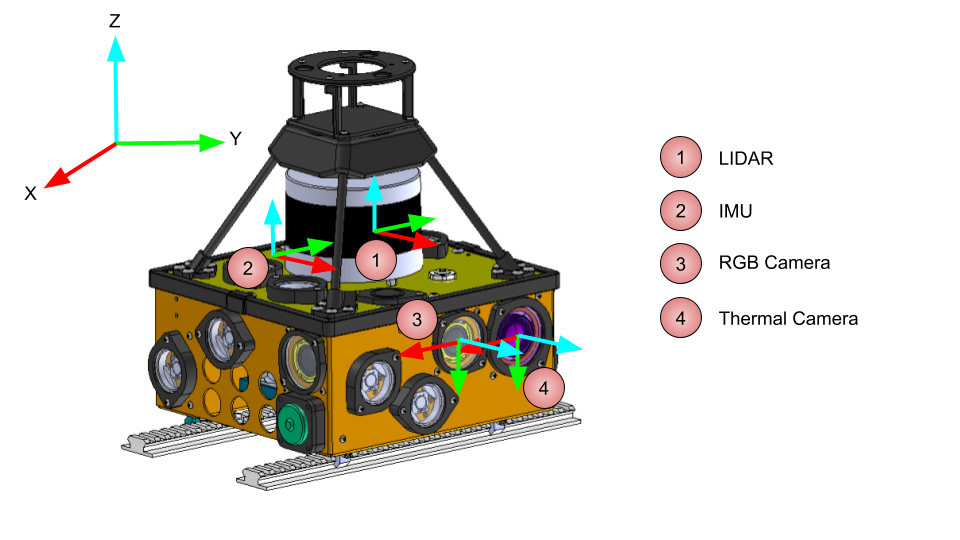
\includegraphics[width=1\textwidth,height=1\textheight,keepaspectratio]{figure/CAD.png}
%     \caption{The CAD model of the payload.} 
%     \label{fig:MMPUG Payload}
%   \end{minipage}
%   \hfill
%   \begin{minipage}[b]{0.4\textwidth}
%     \includegraphics[width=1\textwidth,height=1\textheight,keepaspectratio]{figure/payload.png}
%     \caption{The actual payload.} 
%     \label{fig:MMPUG Payload}
%   \end{minipage}
% \end{figure}


% Need to describe the goal of our payload -- why do we need to design such a payload? ---- sourojit  1-2 sentences 
The sensor payload used for our dataset collection can be seen in Figure\ref{fig:payload}. This payload was designed by the Explorer team during the DARPA Subterranean Challenge and has been assembled rigidly with the purpose of protecting the sensors from external impacts and preventing any internal vibrations. Our sensor payload is equipped with 4 Leopard Imaging RGB monocular cameras, 1 Velodyne puck, 1 Epson M-G365 IMU, and 1 FLIR Boson thermal camera. The payload has an NVIDIA Jetson AGX Xavier as its onboard computer. The specifics for these components can be seen in Table \ref{tab:sensor_overview}.


\begin{figure*} []
   \centering
    \includegraphics[width=\textwidth,height=\textheight,keepaspectratio]{figure/iccv_degraded_scene.pdf}

    \caption{SubT-MRS datasets were collected in various perceptually-degraded environments over different seasons. The scenarios include poor illumination, darkness, and water puddles, in which visual-based sensor fusion methods become unreliable. There are also geometrically degraded environments such as long featureless corridors and steep multi-floors which makes the lidar-based system prone to drift. Also, it includes airborne obscurant conditions such as dust, fog, snow, and smoke in challenging scenes including caves, deserts, long tunnels, and off-road environments.} 
    \label{fig:various_terrains}
\end{figure*}



\begin{figure}[]
    \centering
    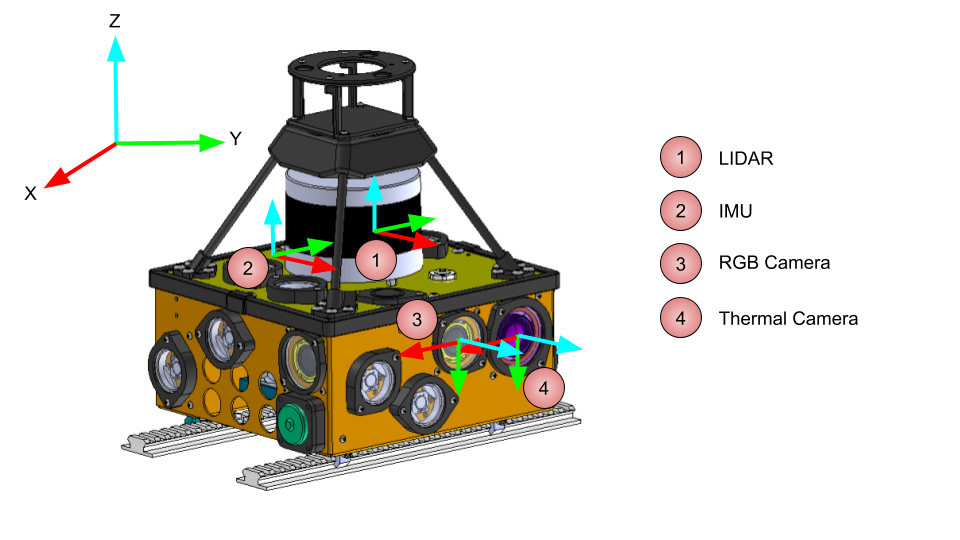
\includegraphics[width=0.95\linewidth]{figure/CAD.png}
    \caption{CAD model of the Payload.}
    \label{fig:payload}
\end{figure}




\begin{table}[]
\resizebox{\linewidth}{!}{
\begin{tabular}{p{1.5cm} l l p{2cm} } 
 \hline
 \textbf{Component} & \textbf{Type} & \textbf{Rate} & \textbf{Characteristics} \\
 \hline
 Lidar & \href{https://velodynelidar.com/products/puck/}{Velodyne VLP-16} & 10Hz & \multirow{2}{2cm}{16 channels, 100m range} \\[0.5cm]
 IMU & \href{https://global.epson.com/products_and_drivers/sensing_system/imu/g365/}{Epson M-G365} & 200Hz & Time Synchronization center \\ 
 RGB Camera & \href{https://www.leopardimaging.com/product/nvidia-jetson-cameras/nvidia-agx-xavier-camera-kits/li-xavier-kit-imx264-x/li-xavier-kit-imx264m12-h/}{LI-Xavier-Kit} & 24Hz & \multirow{2}{2cm}{686$\times$816 pixels}\\[0.8cm]
 Thermal Camera & \href{https://www.flir.com/news-center/camera-cores--components/introducing-the-flir-boson/}{FLIR Boson} & 60Hz & \multirow{2}{2cm}{512$\times$640 pixels}\\[0.8cm]
 Computer & \multirow{2}{2cm}{\href{https://www.nvidia.com/en-us/autonomous-machines/embedded-systems/jetson-agx-xavier/}{Nvidia Jetson AGX Xavier}} & - & \multirow{2}{2cm}{32GB RAM, 8 CPU cores} \\ \hline
\end{tabular}
}

\caption{Overview of sensors on the payload}
\label{tab:sensor_overview}
\end{table}







% Our payload consists of a LIDAR mounted on top of the payload. There are four RGB cameras, one facing the front, two on the lateral sides, and one facing the back. There is one thermal camera facing the front of the payload, placed beside the front-facing RGB camera. The IMU and the onboard computer are placed inside the box. 
% Our payload is  designed to be deployed in a rugged, GPS-denied environment. The components have been added keeping in mind the different scenarios it may encounter, and to provide redundancies in case of sensor failure.
% The payload consists of one each of LIDAR, IMU, thermal camera, and four RGB cameras shown in Fig.\ref{fig:payload}, which are rigidly assembled in a case. It also contains an onboard computer for running autonomy and SLAM algorithms. Table \ref{tab:sensor_overview} mentions all the components in our payload. The specifications of the components are as follows:
%     \begin{itemize}[noitemsep,topsep=0pt]
%         \item The payload is equipped with a Velodyne VLP-16 LIDAR. It is a 16-channel LIDAR at 10Hz. The vertical FoV is $-15^{\circ}$ to $+15^{\circ}$. This LIDAR has a range of 100m with a range accuracy of $\pm3$cm.
        
%         \item The IMU mounted on the inside of the payload is an Epson M-G365 IMU, which operates at 200Hz. The other sensors are synchronized with respect to the IMU.
        
%         \item The four cameras mounted on the payload are Li-Xavier Kit from Leopard imaging. Each camera has a horizontal FoV of $37^{\circ}$ and provides images of 686$\times$816 pixels at a frequency of 24Hz.
%         % The RGB camera used for state estimation is \href{https://www.leopardimaging.com/product/nvidia-jetson-cameras/nvidia-agx-xavier-camera-kits/li-xavier-kit-imx264-x/li-xavier-kit-imx264m12-h/}{LI-XAVIER-KIT-IMX264M12} from Leopard imaging, which runs at a rate of 24Hz and the image resolution used in $686\times816$ pixels. 
        
%         % \item The thermal camera used in the payload is a FLIR Boson camera that runs at a frequency of 60Hz and outputs an image of 512$\times$640 pixels. 
%         \item The onboard computer in use is an Nvidia Jetson AGX Xavier module. It has a memory of 32GB and 8 CPU cores, 512 Nvidia CUDA cores, and 64 Tensor cores. On this computer, all the autonomy and SLAM algorithms can run online.
%     \end{itemize}

    % \begin{itemize}
    %     \item The LIDAR is a 16 channel \href{https://velodynelidar.com/products/puck/}{Velodyne VLP-16}, which runs at a rate of 10Hz. It has a field of view of $30^{\circ}$ and a range of 100m. The range accuracy is $\pm3$cm.
        
    %     \item The IMU used is \href{https://global.epson.com/products_and_drivers/sensing_system/imu/g365/}{Epson M-G365}. It runs at a rate of 200Hz.
        
    %     \item The RGB camera used for state estimation is \href{https://www.leopardimaging.com/product/nvidia-jetson-cameras/nvidia-agx-xavier-camera-kits/li-xavier-kit-imx264-x/li-xavier-kit-imx264m12-h/}{LI-XAVIER-KIT-IMX264M12} from Leopard imaging, which runs at a rate of 24Hz and the image resolution used in $686\times816$ pixels. 
        
    %     \item The thermal camera is \href{https://www.flir.com/news-center/camera-cores--components/introducing-the-flir-boson/}{Boson FLIR}. It runs at a rate of 60Hz and provides an image of $512\times640$ pixels resolution.
        
    %     \item The onboard computer in use is a \href{https://www.nvidia.com/en-us/autonomous-machines/embedded-systems/jetson-agx-xavier/}{Nvidia Jetson AGX Xavier} computer. All the autonomy and SLAM algorithms run on this computer online.
    % \end{itemize}
    % \item Description of the CPU, GPU--\\
    % We are using Nvidia Jetson AGX Xavier.






% \begin{center}
% % \begin{tabular}{ l l l l } 
% \begin{table}[h!]
% \begin{tabular}{p{1.5cm} l l p{2cm} } 
%  \hline
%  \textbf{Sensor} & \textbf{Type} & \textbf{Rate} & \textbf{Characteristics} \\
%  \hline
%  Lidar & Velodyne & 10Hz & \multirow{4}{2cm}{16 channels, 100m range, $30^{\circ}$vertical FoV}\\\\\\ \\
%  IMU & Epson & 200Hz & All sensors synchronised wrt IMU \\ 
%  RGB Camera & Leopard imaging & 24Hz & \multirow{2}{2cm}{686$\times$816 pixel}\\
%  Thermal Camera & Boson FLIR & 60Hz & \multirow{2}{2cm}{512$\times$640 pixel}\\
%  \hline
% \end{tabular}
% \caption{Overview of sensors on the payload}
% \label{tab:sensor_overview}
% \end{table}
% \end{center}
\subsection{Time Synchronization of Sensors}

\begin{figure}[!ht]
    \centering
    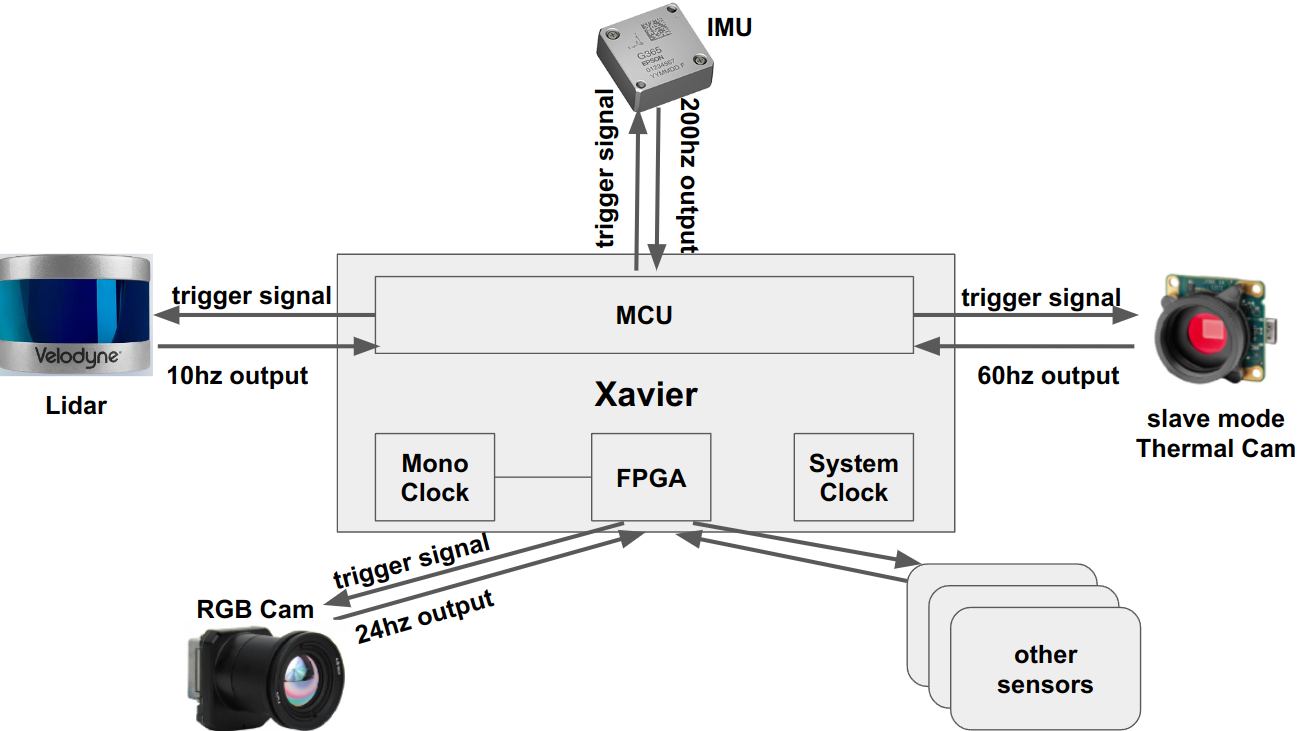
\includegraphics[width=1\linewidth]{figure/sync_pic.png}
    \caption{Sensor hardware time synchronization paradigm}
    \label{fig:synchronization}
\end{figure}


Time synchronization plays a critical role in any multi-sensor system and we achieve that using the ``pulse per second (PPS)'' technique. All the sensors sync to the CPU clock on the onboard computer, as can be seen in Figure \ref{fig:synchronization}. The IMU, LiDAR, and thermal camera directly use the CPU clock, whereas the 4 RGB cameras are synchronized using an FPGA board. Our experiments revealed that the time synchronization gap between any two sensors is not greater than 3ms.


% Our system contains different types of sensors including  RGB cameras, thermal cameras, Lidar, and IMU. We use the same CPU clock to generate all the sensor timestamps. Once every second, the CPU produces pulse signals that synchronize the thermal camera, IMU and Lidar. As for the RGB camera, it is triggered by a specially-designed FPGA module.
% %, which can be taken as a more accurate CPU clock for cameras. 
% %Through experiments, we have achieved hardware synchronization between the RGB camera and IMU. 
% Our experiments show that the synchronization between the thermal camera and IMU is within 3 ms. The system structure is shown in Fig. \ref{fig: synchronization}. 


\subsection{IMU Calibration}

% A 90 min sequence of IMU data was collected on a stationary
% flat surface. We adopted the Allan Variance estimation method5
% to compute the angle random walk, bias instability, and random
% walk for the gyroscope and the velocity random walk, bias
% instability, and random walk for the accelerometer. This IMU
% rosbag is provided with the dataset for the user’s convenience.

%https://github.com/gaowenliang/imu_utils
We use the M-G365 inertial sensor\footnote{\href{https://global.epson.com/products\_and\_drivers/sensing\_system/imu/g365/}{https://global.epson.com/products\_and\_drivers/sensing\_system/imu/g365/}} on our platform and calibrate it to reduce bias instability and drift. We employ an Allan variance\cite{4404126} based tool\footnote{\href{https://github.com/gaowenliang/imu\_utils}{https://github.com/gaowenliang/imu\_utils}}
%to estimate the white noise angle random walk, and the bias instability of the angular velocity from gyroscope data as well as the white noise angle random walk, and bias instability of the accelerometer data present in the IMU.
to estimate the white noise angle random walk and bias instability for both the gyroscope and accelerometer data.
To this end, we collect a 1-hour IMU data sequence on a flat and stationary surface, consistent with other datasets like \cite{zhang2021multi}. The same is made available in our dataset to the user. The IMU-LiDAR calibration is done using CAD models, the data for which will be made available to the user.

% \begin{itemize}
%     \item Describe how you calibrate our IMU sensors 
% \end{itemize}

\subsection{RGB Camera Calibration}

We use an open-source calibration toolbox, Kalibr\footnote{\href{https://github.com/ethz-asl/kalibr}{https://github.com/ethz-asl/kalibr}} for the intrinsic and extrinsic calibration of the RGB camera. The camera is extrinsically calibrated to the IMU. For this purpose, we use a 7$\times$9 checkerboard, the omnidirectional camera model, and the radial-tangential distortion model. A $60s$ random-motion video is used for the calibration, which will be provided to the user along with other parameters.


% Accurate intrinsic calibration is vital for achieving the best performance of the system. We used a standard checkerboard calibration for camera intrinsic calibration and the open-source calibration toolbox \textbf{Kalibr} to compute the intrinsic parameters for our camera. The calibration target used was a 7$\times$9 checkerboard, where the size of each cell was 4.5 inches. The camera model used was an omni-radtan model with equidistant distortion. A 60 sec video clip of the calibration board was recorded with our cameras. This was then fed into the Kalibr toolbox to get the intrinsic calibration results.


% For intrinsic calibration, the Kalibr software \textbf{give ref} was used. This open-source software is capable of computing the cave. ras' intrinsic and extrinsic parameters. For visual calibration, a standard checkerboard was used. The images of the checkerboard were collected from different orientations and locations. These parameters were then fed into the \textbf{kalibr} software to get the intrinsic camera parameters.

% \begin{figure}[!tbp]
%   \centering
%   \begin{minipage}[b]{0.4\textwidth}
%     \includegraphics[width=1\textwidth,height=1\textheight,keepaspectratio]{figure/RGB image.png}
%     \caption{The RGB image as seen by the front camera} 
%     \label{fig:MMPUG Payload}
%   \end{minipage}
%   \hfill
%   \begin{minipage}[b]{0.4\textwidth}
%     \includegraphics[width=1\textwidth,height=1\textheight,keepaspectratio]{figure/Thermal image.png}
%     \caption{The Thermal image as seen by the thermal camera} 
%     \label{fig:MMPUG Payload}
%   \end{minipage}
% \end{figure}

% \begin{figure}[ht!]
%     \centering
%     \includegraphics[width=1\linewidth]{figure/calibration board.png}
%     \caption{The images as seen by the RGB and thermal cameras are shown on the left and right respectively}
%     \label{fig:thermal image}
% \end{figure}




% \begin{figure*}
%   \centering
%     \includegraphics[width=0.5\textwidth,height=0.5\textheight,keepaspectratio]{figure/RGB image.png}
%     \caption{The RGB image as seen by the front camera.} 
%     \label{fig:MMPUG Payload}
% \end{figure*}

% \begin{figure*}
%   \centering
%     \includegraphics[width=0.5\textwidth,height=0.5\textheight,keepaspectratio]{figure/Thermal image.png}
%     \caption{The Thermal image as seen by the front camera.} 
%     \label{fig:MMPUG Payload}
% \end{figure*}

\subsection{Thermal Camera Calibration} 

Calibrating a thermal camera follows a procedure similar to that of an RGB camera, with the addition of an image processing task that requires obtaining a thermal calibration image with good contrast. This can be challenging, but we achieved it by heating a 7$\times$9 chessboard under sunlight and feeding an inverted image from the recording into the Kalibr toolbox. Like the RGB camera, the thermal camera is also extrinsically calibrated to the IMU. This process uses a $60s$ random-motion clip, which we provide to the user along with other essential parameters.


% Calibrating a thermal camera is challenging because a normal checkerboard image with no difference in temperature will show up as a blank board to a thermal camera. To obtain a temperature gradient in the shape of the chessboard's pattern, we choose to heat up the board under sunlight until the thermal camera has a clear picture of the chessboard's pattern. The pattern of the chessboard has 7 rows and 9 columns of grids and both black and white grids have 11.8cm edges. In experiments, the thermal image of the heated checkerboard showed white patches as black and black patches as white. In order to make these thermal images compatible with the calibration packages, we rescaled the raw image data to 8bits grayscale images and manually reverse the lightness to make the white patches have a lighter color and the black patches a deeper color. The images of the checkerboard were collected from different orientations and locations. Finally, they were fed into the \textbf{Kalibr} software to calculate the intrinsic camera parameters. To be more specific, we used a pinhole model and a padding size of 0.06 for calibration.  

% Calibrating a thermal camera is challenging because a normal checkerboard image with no difference in temperature will show up as a blank board to a thermal camera. To get a temperature difference in the shape of the chessboard's pattern, we choose to heat up the board with sunlight until the thermal camera has a clear picture of the chessboard's pattern. In addition, the checkerboard we use is made of foam and we can ignore the deformation caused by temperature variation. The pattern of the chessboard has 7 rows and 9 columns of grids and both black and white grids have 11.8cm edges. In experiments, the thermal image of the heated checkerboard showed white patches as black and black patches as white. In order to make these thermal images compatible with the calibration packages, we rescaled the raw image data to 8bits grayscale images and manually reverse the lightness to make the white patches have a lighter color and the black patches a deeper color. The images of the checkerboard were collected from different orientations and locations. Finally, they were fed into the \textbf{Kalibr} software to calculate the intrinsic camera parameters. To be more specific, we used a pinhole model and a padding size of 0.06 for calibration.  



% \subsection{Lidar Calibration}

% \begin{figure}[]
%     \centering
%     % \includegraphics[width=0.7\textwidth, height=0.7]{figure/autocalar.png}
%     \includegraphics[scale=0.3,keepaspectratio]{figure/autocalib with green bar.png}
%     \caption{Extrinsic calibration using GICP}
%     % \caption{Overview of Auto Calibration between multi robots. The lead robot shares its local map from the start location with the base station (shown by the red arrow). This will be used as a reference by other robots to align their local map. Each of the remaining robots moves to the start location and requests the reference map from the base station (shown by the blue arrow). Once received, it aligns its local map to the reference map. This alignment is achieved by performing GICP between the reference map and the local map of the robot.  }
%     % \caption{Overview of Extrinsic Calibration between multi robots. At least one robot is calibrated using the total station via least-squares registration, while also sharing a local map to the base station. Subsequent robots may request this map from the base station and perform alignment with respect to its own local map}
%     \label{fig:autocalib}
% \end{figure}
\subsection{Extrinsic Calibration for Multiple Robots}\label{sec:extrinsic_calib_robots}
Collaborative tasks require multiple robots to operate in a common frame of reference. Our procedure to create this involves the usage of Generalized-ICP (GICP)\cite{segal2009generalized} and is two-fold. In the first step, one robot shares its map from a feature-rich location to a base station. In the second step, the remaining robots take turns solving a GICP, in the same feature-rich location as the first robot and obtain a frame transformation from its own to the first robot. All the robots end up in a common frame after this procedure and build their map further using Super Odometry\cite{zhao2021super}. We will provide a graphic and mathematical description of this process in the supplemental material.


% In the first step, a lead robot is taken to the calibration position and it creates a local point cloud map of its surroundings. This map is then shared with the base station. This is the reference map that other robots will use to calibrate. The lead robot is then moved from the calibration position to make way for other robots. 

% In the second step, subsequent robots are taken to the calibration position to create a local map of their surrounding. The reference map is shared from the base station with the robot. A GICP registration between the reference map and the local map of the robot is computed. This transformation is used to align the map of this robot to the reference map. After registration, the robot is moved from the calibration position, and the steps are repeated for the remaining robots

% This method ensures effective collaboration between the robots by ensuring that they all operate in the same spatial orientation, enabling them to complete the task with precision and accuracy. A visual description of this procedure is provided in Fig 
% \ref{fig:autocalib}


% To finish a collaborative task, multiple robots need to operate in a common frame of reference. This is achieved by computing the relative rigid-body transformation of the robots with respect to a pre-specified reference frame. We achieve this using a procedure called Auto Calibration (AC), based on Generalized-ICP (GICP) \cite{segal2009generalized}. The AC procedure has two steps. In the first step, a lead robot moves to the calibration position and captures its surroundings with the point cloud, after which, it shares this map with the base station. In the second step, each subsequent robot is taken to the calibration position. It captures its local map and requests the reference map from the base station. Finally, a GICP registration between the reference map and the local map is computed. This result will align each robot with the reference frame created by the first robot. Once complete, the robot moves from this position and the steps are repeated for the remaining robots. A description of the information flow is given in Fig \ref{fig:autocalib}.

% With AC, the inter-robot alignment depends on the environment in the base station area. This is not an issue because usually this is known and can be chosen in a manner that benefits the process. Additionally, by using the GICP process, it allows for good results even with a rough positioning of the robots in the calibration location, which is typically accomplished with the teleoperation of the robots. 
% The first being the generation of the reference map, 
% ref \ref{alg:Generating Reference Map}
% where the lead robot shares its local map with the base station. And the second step, 
% ref \ref{alg: Calibrating other robots}, 
% is where the other robots request this reference map from the base station and compute the transform. 


% To achieve a shared task, multiple robots must be able to operate in a common frame of reference. In the Subt Challenge, we used \textit{DARPA frame}, which was used to express the location of the artifacts. In Tunnel and Urban Circuits, our team used a Total Station (TS) to obtain a 6 degree-of-freedom transformation $\mathbf{T}^d_m$  that aligned the mapping frame $m$ of each robot with the DARPA frame $d$. This process was time-consuming since it required an experienced TS operator to coordinate with the base station operator to obtain two control points for each robot, by moving them as much as possible within the staging area.



% The extrinsic calibration among robots is performed by a procedure we call as AutoCalibrattion. At its core, the robots perform ICP between their own map and a reference map, shared by another robot, to get the transformation matrix. The robots should be placed in approximately the same location before calibrating the maps.
% The steps for the AutoCalibration are as follows:

% \begin{algorithm}
% \caption{Generating Reference Map}
% \label{alg:Generating Reference Map}
% \begin{algorithmic}[1]
%     % \State \textbf{Generate reference map}
%     % \State \textbf{Inputs: }Lead robot, starting location
%     % \State \hskip1.0em Take the lead robot to the start location
%     % \State \hskip1.0em Capture the map and share it with base station
%     % \State \hskip1.0em Move the robot from the start location
    
%     \State \textbf{Inputs: }Lead robot, Basestation, starting location
%     \State \textbf{Outputs: }Reference map
%     \State Take the lead robot to the start location
%     \State Capture the map, this is the \textbf{reference map}
%     \State Share map with the base station
%     \State Move the robot from the start location

% \end{algorithmic}
% \end{algorithm}

% \begin{algorithm}
% \caption{Calibrating other robots}
% \label{alg:Calibrating other robots}
% \begin{algorithmic}[1]
%     % \State \textbf{Generate reference map}
%     \State \textbf{Inputs: }Set of robots R, Basestation, start location of the lead robot, reference map
%     \State \textbf{Outputs: }Relative transformation between robots, Calibrated maps on all robots
%     \For{each robot in R}
%     \State Move robot to start location
%     \State Capture its map
%     \State Request reference map form Basestation
%     \State Initiate AutoCalibration
%     \State Move robot from the start location
%     \EndFor

% \end{algorithmic}
% \end{algorithm}

% \begin{itemize}
%     \item 1. Take the first robot to the start location and capture its map. This map will be used as the reference for all other robots. Remove the robot from the start location.  other robots.
%     \item 2. After capturing the map, share it with all.
%     \item 3. Bring the next robot to the start location and capture its map. This robot should be in approximately the same location and orientation. Remove the robot from the start location and initiate autocalibration.
%     \item 4. For other robots perform step 3.
% \end{itemize}
% For the autocalibration to give good results, the following conditions should be met:
% \begin{itemize}
%     \item The start locations should be in a feature-rich environment. 
%     \item All the robots should have a similar perspective of the environment, i.e. The height, roll, pitch, and yaw should be similar.
%     \item The robots should be placed in approximately the same start location and have a similar orientation.
% \end{itemize}

\begin{figure*}[ht!]
    \centering
    % \includegraphics[width=0.7\textwidth, height=0.7]{figure/autocal.png}
    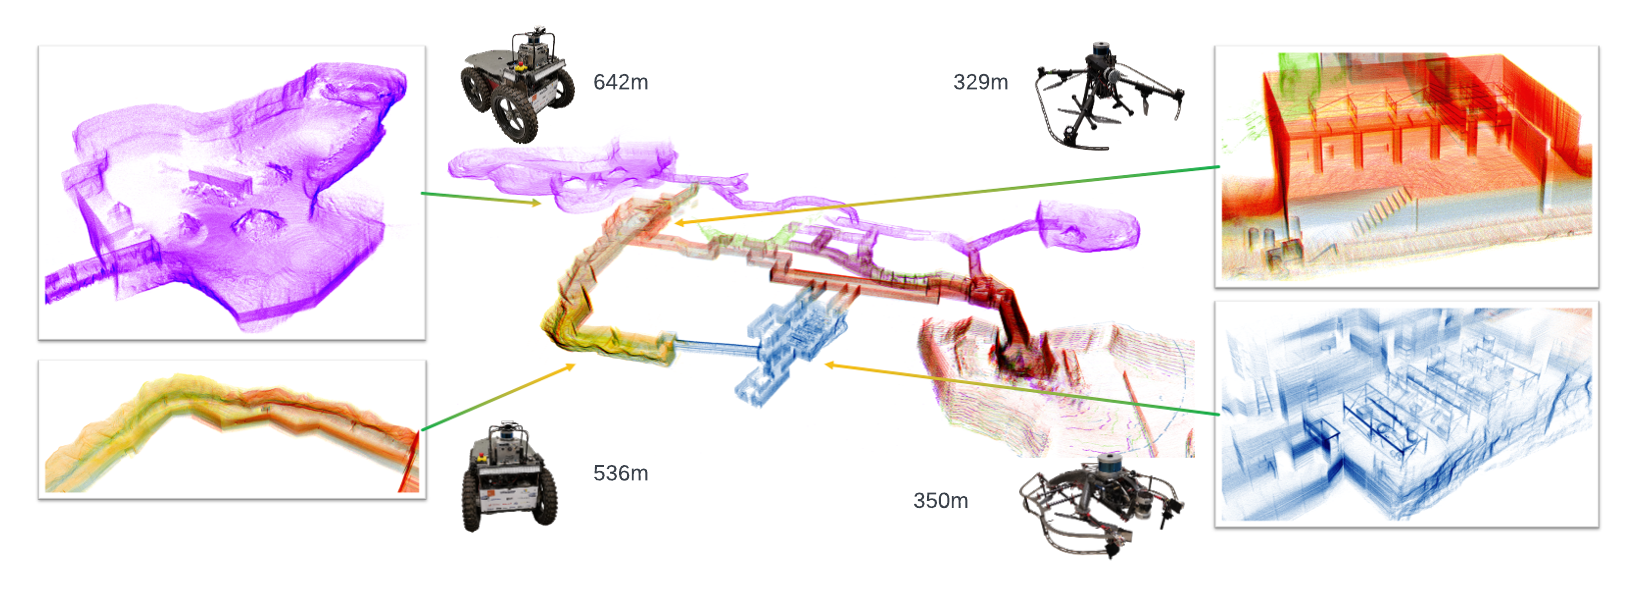
\includegraphics[width=0.9\linewidth]{figure/subt_v2.png}
    \caption{Point cloud of the Subt-MRS dataset, generated by Super Odometry\cite{zhao2021super}. Different colors represent point clouds collected by different robots. }
    \label{fig:subt_pointcloud}
\end{figure*}

%------------------------------------------------------------------------

\section{Dataset}\label{sec:dataset}

Our dataset was recorded in the form of ROS bags, in diverse locations including rural and urban areas, and structured and unstructured sites, to provide varying levels of challenge for modern SLAM algorithms. The data contains multi-modal and sensor-degraded data and was recorded on multiple robots with varying kinematic profiles. The locations range from university campuses to caverns, buildings, and off-road areas (as shown in Figure \ref{fig:various_terrains}). Here we briefly discuss our dataset in the following sub-sections. The detailed specifications of our dataset are further listed and discussed comprehensively in the supplementary material.

% All the data is provided on the SuperOdometry website \footnote{\href{https://superodometry.com/}{https://superodometry.com/datasets.com}}


% Our dataset is packaged as shown in table \textbf{(give ref)}

% \begin{itemize}
%     \item Talk about data recording formats - rosbag, las etc
%     \item Talk about the amount of data
%     \item Table to show different categories of data 
% \end{itemize}

\subsection{Multi Modal Dataset}

% Describe that our dataset is very unique and contains multi-modal spectra from lidar to thermal

Our dataset incorporates data from RGB cameras, thermal camera, LiDAR, and IMU, making it a multi-modal dataset. The majority of our dataset incorporates multi-modal data, recorded on different vehicles like the RC car, legged robot, and drones. This dataset has been collected in varied locations like caves, buildings, and university campus areas.
%  The major challenge is estimating the uncertainty of each sensor and seamlessly switching between them. To foster research in this area, the Subt-MRS dataset contains data from four different sensors: LiDAR, IMU, RGB and Thermal camera. It includes more sensors than other published datasets, as shown in Table~\ref{tab:datasets}. 
%We aim to make our dataset support researches of SLAM algorithms with different combinations of the four sensors included. 




% \begin{figure*}[tbh]
%     \centering
%     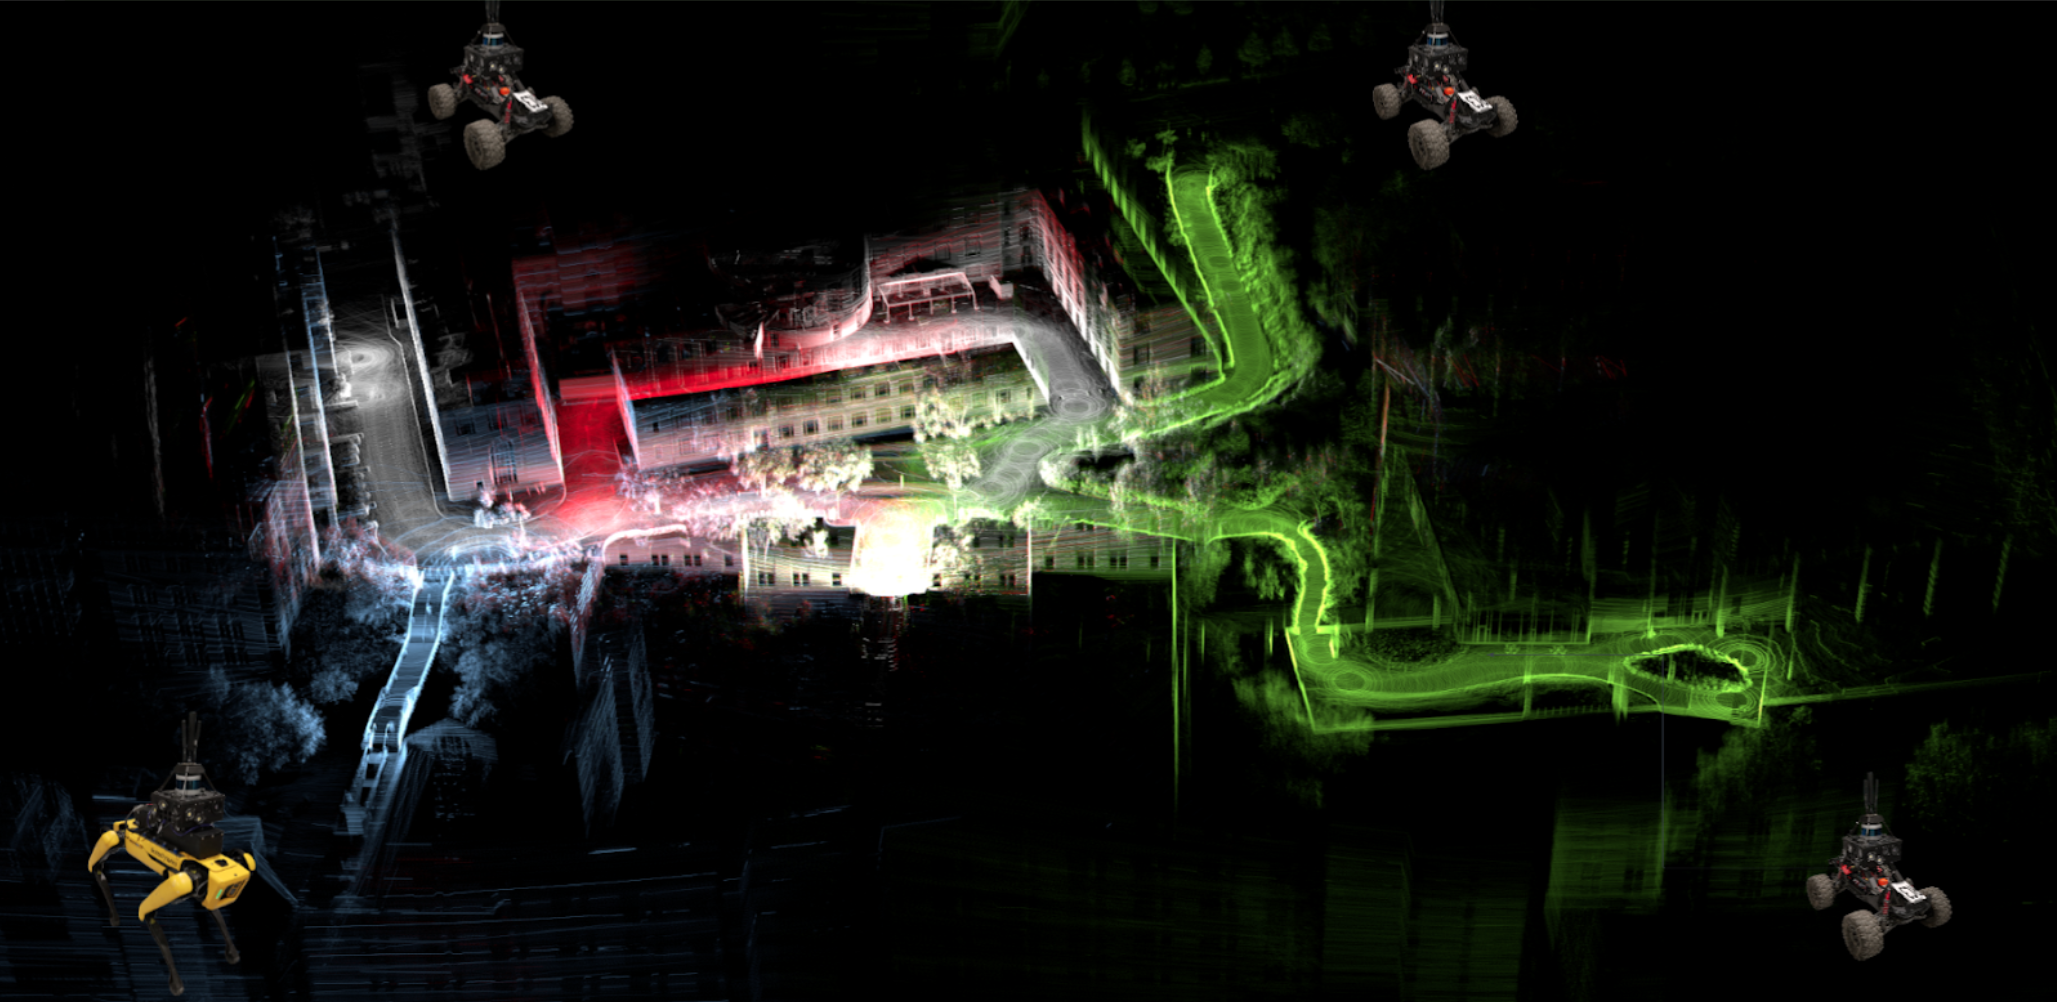
\includegraphics[scale=0.2]{figure/nsh_multi_robot_run.png}
%     \caption{Mapping result from multi-robot dataset}
%     \label{fig:nsh_multi_robot_mapping}
% \end{figure*}

\subsection{Multi Robot Dataset}

Multi-robot SLAM(MR-SLAM) has garnered increasing attention in recent years due to its immense applications ranging from warehouse management, and autonomous truck fleets \cite{lajoie2022} to search and rescue \cite{9220149}. 

To this end, a lot of focus is being put on building systems such as \cite{https://doi.org/10.48550/arxiv.2205.13135}  to tackle the problem of MR-SLAM. This naturally warrants a reliable multi-robot dataset, yet, as is visible from \ref{Tab:dataset_compare} none of the publicly available datasets provide detailed multi-robot data. To enable research and development of MR-SLAM systems,  we are the first ones to provide \textbf{time} and \textbf{frame-synchronized sensor data} from 3 RC cars and a legged robot in a diverse environment. This data has been collected in the campus area, hospital building, and caves.

% \textbf{Table~\ref{tab:multi_robot_data} shows the data provided for all 4 robots.where is table?}

% A detailed topic list is given in Appendix \# \textbf{\textit{(needed?)}}. All the robots in this dataset used SuperOdometry \cite{zhao2021super} as their SLAM system.

% As mentioned in \cite{lajoie2022}, multi-robot SLAM (MR-SLAM) or collaborative SLAM (C-SLAM) has applications ranging from warehouses to autonomous truck fleets to planetary exploration. Solving large-scale mapping and localization problems warrants the use of MR-SLAM techniques. To cater to the analysis of such systems, section \#this - \#that of SubT-MRS provides time and frame-synchronized data from 4 robots (3-wheeled + 1-legged). As can be noted in Table \ref{tab:datasets} none of the datasets provide multi-robot data. There, SubT-MRS is the first one to provide data for multi-robot SLAM analysis. Table~\ref{tab:multi_robot_data} shows the data provided for all 4 robots.
% %We facilitate such analysis by developing a dataset produced by compiling individual data from 4 robots in time and frame synchronized runs, packaging the information listed in table \ref{tab:multi_robot_data}.
% A detailed topic list is given in Appendix \# \textbf{\textit{(needed?)}}. All the robots in this dataset used SuperOdometry \cite{zhao2021super} as their SLAM system.


\subsubsection{Synchronization}
To get the best performance out of a multi-robot system, it is necessary to have all the robots operate in the same time and world frame. The time across all the robots is synchronized with respect to a common base station clock over Secure Shell. All the robots are aligned to the world frame using the calibration techniques explained in section \ref{sec:extrinsic_calib_robots}.

% Having all the sensor data in a unified time and world frame is a necessity for MR-SLAM systems, which is also a major challenge in developing a multi-robot dataset. To achieve time synchronization between robots we sync their clocks using a base station clock, over Secure Shell. The world frames for all the robots are synchronized using Auto Calibration, as explained in section \ref{sec:extrinsic_calib_robots}.

% \begin{table}
% \centering
% \begin{tabular}{|c|c|c|}
%      \hline
%      \textbf{Type} & \textbf{Frequency(Hz)} & \textbf{Robots}\\
%      \hline
%      LiDAR & 10 & All \\
%      \hline
%      RGB Image & 24 & All \\
%      \hline
%      IMU data & 200 & All \\
%      \hline
%      SNR & 20 & All\\
%      \hline
%      Static Transform & -- & All\\
%      \hline
% \end{tabular}
% \caption{Data in multi-robot rosbags}
% \label{tab:multi_robot_data}
% \end{table}

% \subsubsection{Communication Signal Strength}

% As explained in \cite{lajoie2022}, communication constraints play a significant role in MR-SLAM systems. They vary from packet sizes to bandwidth availability and have been utilized in different ways in the MR-SLAM. We provide Signal-to-Noise Ratio(SNR) values in our dataset to indicate the communication constraints between the robots. SNR value is given as
% % $$SNR = \frac{P_{signal}}{P_{noise}}$$
% \begin{equation}\label{eq:SNR_formula}
%     \mathrm{SNR} = \frac{P_{signal}}{P_{noise}}
% \end{equation}
% % $SNR = \frac{P_{signal}}{P_{noise}}$
% \begin{equation}\label{eq:snr_decode}
%     \begin{aligned}
%     % SNR = (TX\_POWER + TX\_GAIN + RX\_GAIN)\\ - PATH\_LOSS + NOISE\_FLOOR
%     \mathrm{SNR} = (TX_{power} + TX_{gain} + RX_{gain})\\ - Path_{loss} + Noise_{floor}
%     \end{aligned}
% \end{equation}
% In a general sense, the SNR can be decoded as given in equation \ref{eq:snr_decode}. The SNR value encodes multiple wireless communication information such as bandwidth availability, packet sizes, packet rates, and distance. Therefore, they can be used to measure the network strength to ensure seamless data flow for multi-robot SLAM optimizations.
% \textbf{As shown in Figure \ref{fig:mpu5}, we use Persistent Systems MPU5 radios.} Using the standard WebSocket API on these smart radios, we can query the SNR values between any robot and its neighbors. Internally, these radios calculate the SNR values by packet transfer analysis, as shown in equation \ref{eq:SNR_formula}.

% \begin{figure}[th!]
%     \centering
%     \includegraphics[scale=0.5]{figure/mpu5.png}
%     \caption{Persistent Systems MPU5 radio}
%     \label{fig:mpu5}
% \end{figure}

% As mentioned in section \ref{sec:extrinsic_calib_robots}, we obtain the initial robot frame transformations using Auto-Calibration. The robots are then driven onto their own paths. Figure \ref{fig:nsh_multi_robot_mapping} shows the results of the multi-robot mapping achieved in front of the Newell-Simon Hall at Carnegie Mellon University.

% \begin{figure}[h!]
%     \centering
%     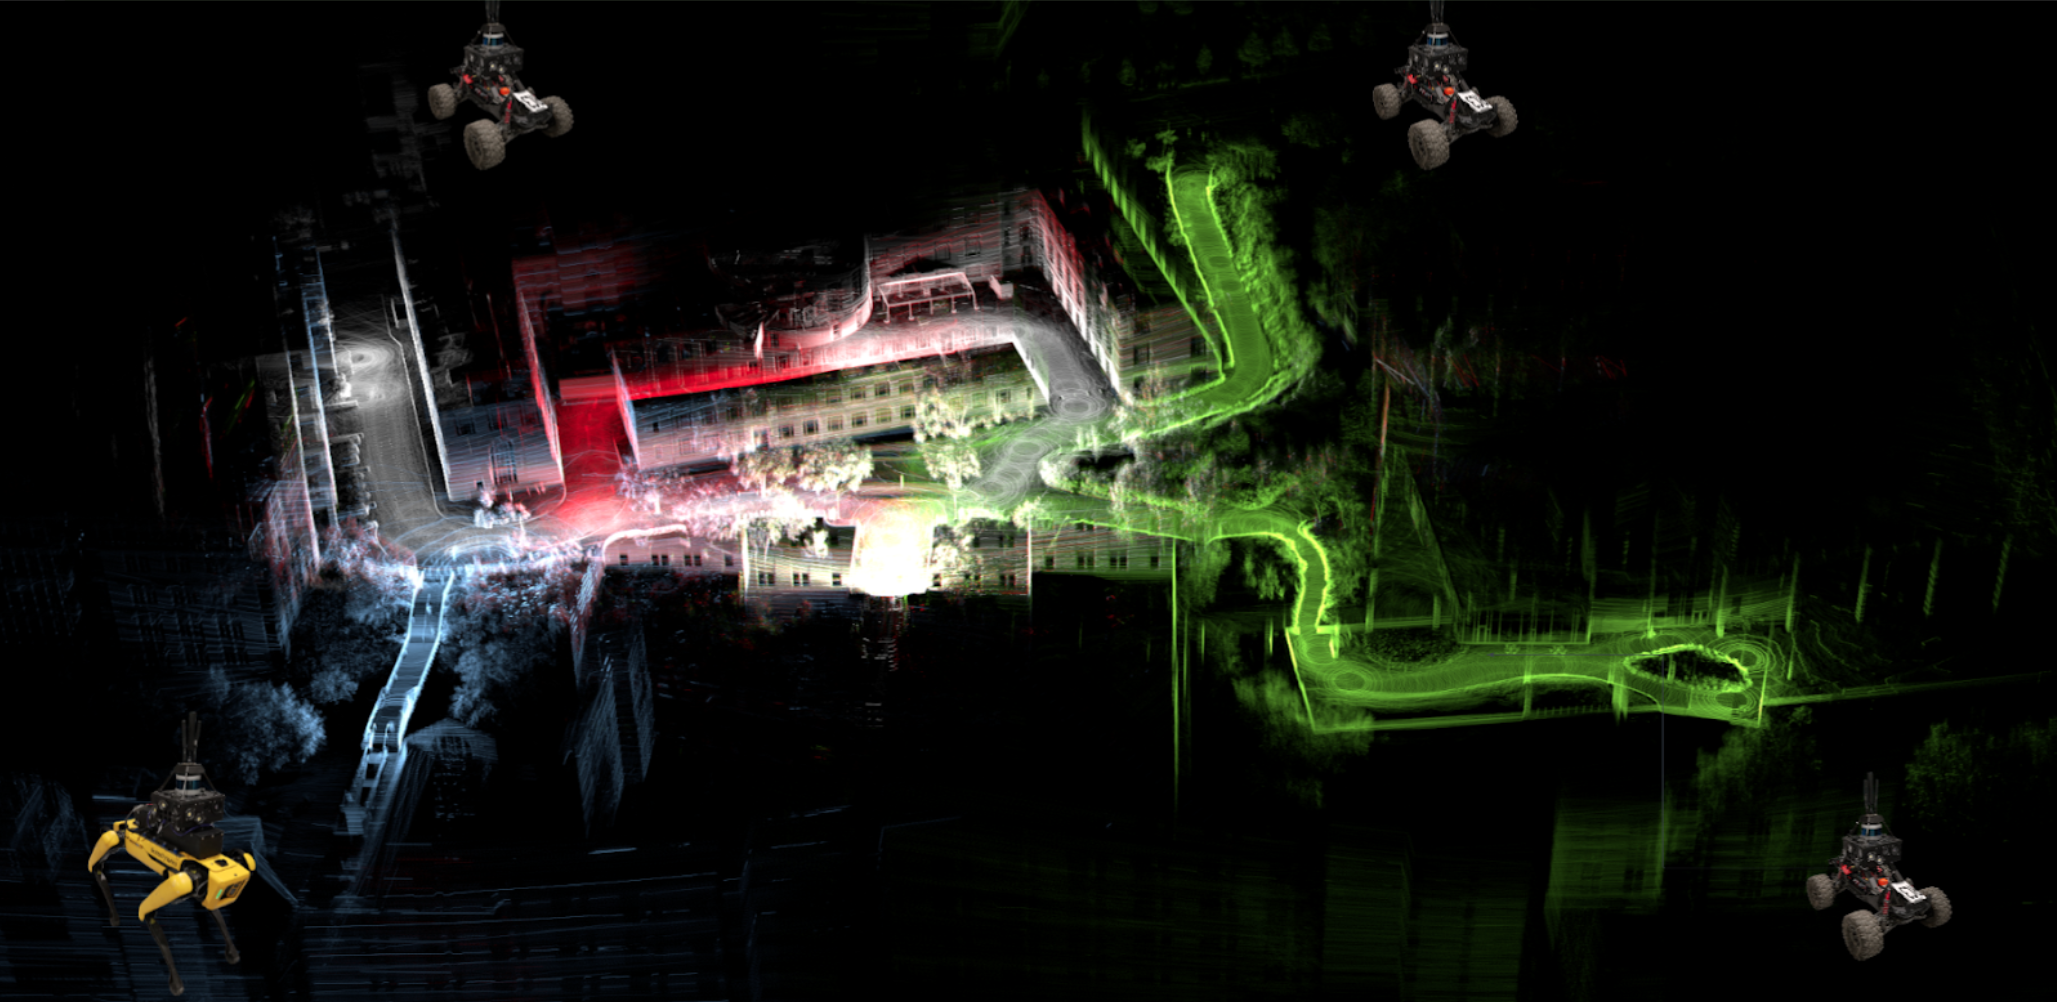
\includegraphics[width=1\linewidth]{figure/nsh_multi_robot_run.png}
%     % \includegraphics[width=1\linewidth]{figure/subt.png}
%     \caption{Mapping result from multi-robot dataset}
%     \label{fig:nsh_multi_robot_mapping}
% \end{figure}

% \subsubsection{Kinematic Profiles from Different Robots}

% Our dataset involves robots with different kinematic profiles. It includes data from RC cars (wheeled car-like robots) and a Boston Dynamics Spot (four-legged robot). RC cars give fast-moving data whereas the Spot is capable of traversing staircases. Different locomotion capabilities result in diverse speeds and environments in a single run, which can be challenging for MR-SLAM solutions. Multiple locomotion modalities also allow us to include multi-floor data in a single run. The different motion capabilities for the robots can be seen in Fig. \ref{fig:autocalib}.
% The different robot kinematic profiles can be seen in table \ref{tab:robot_motion_charac}


% \begin{table}
% \centering
% \begin{tabular}{|c|c|c|}
%      \hline
%      \textbf{Robot Type} & \textbf{Max Speed (m/s)} & \textbf{Muti-Floor}\\
%      \hline
%      RC Car & 4 & No\\
%      \hline
%      Legged Robot & 1.5 & Yes\\
%      \hline
%      Canary Drone & 2 & Yes\\
%      \hline
% \end{tabular}
% \caption{kinematic profiles from different robots}
% \label{tab:robot_motion_charac}
% \end{table}


% \subsubsection{Collaborative Behavior with Different Robots}



\subsection{Multi Degraded Dataset}

% Sensor fusion algorithms in SLAM are built to sustain sensor degradation.
% SubT-MRS includes runs containing multiple data degradation sources to provide good analyses of such systems.
Subt-MRS includes different sensor degradation categorized as visually degraded, geometrically degraded, and simultaneously degraded.
% These are challenging for multi-modal SLAM as they involve areas with single or multiple sensor failures. 
In the following sections, we discuss the different types of sensor degradation in our dataset.

\subsubsection{ Visually Degraded}
% Visual degradation happens when the RGB camera cannot extract an adequate amount of good-quality features, which generally happens in areas lacking RGB color texture. 
% We collect visually degraded data from caves and buildings.
Visual degradation happens in areas with low visual textures like low-lit areas, smoke/fog, etc.
In this dataset, we collect the data from subterranean and indoor environments, e.g., corridors.
% Visual degradation when the environment does not allow for the RGB sensor to detect a visual gradient. This typically happens in low-light environments or in the absence of visual texture in the observed scene, such as white walls or smoke. Without enough contrast for feature extraction, these kinds of environments are challenging for visual odometry.
% B, J, L, M, N, O, U

\begin{enumerate}[label=(\alph*)]
    \item \textbf{Low light and Darkness:} Our dataset includes several sequences in dim environments from the hospital building as well as the caves. 
    The images A-F in Figure \ref{fig:various_terrains} provide a glimpse of the environment.
    % Our dataset includes several runs in dark environments where the RGB camera is able to extract very minute amount of features and most visual SLAM algorithms fais in these regions
    % Data were collected indoors in caves or with no environmental light. The robot was equipped with onboard LED lighting. Mixed geometry features on the walls.
    \item \textbf{Smoke and Dust:} Our dataset includes runs in smoke-filled areas in the hospital and caves. The images M-N in figure \ref{fig:various_terrains} show snapshots from these runs.
    
    
    % Data was collected in caves. The environment was full of manually generated smoke. Mixed geometry features on the walls.
\end{enumerate}

\subsubsection{ Geometrically Degraded}
Geometric degradation relates to when environmental degradation of the LiDAR sensor either due to lack of structural features like planes, points, lines, etc, or due to LiDAR range deficit in big parking areas and long corridors leads to LiDAR odometry being unconstrained.
% Geometric degradation happens when the environment does not provide enough landmarks that may be used as features in LiDAR odometry. For example, long man-made corridors typically provide no geometric features that can constrain the forward direction of motion. Other scenarios can also occur if the sensor fails to capture points from the floor and/or the ceiling. In this case, the up/down direction becomes unconstrained. 

%lucas wrote this


\begin{enumerate}[label=(\alph*)]
    \item \textbf{Long corridor} \\
    In a featureless long corridor environment, the LiDAR range falls short. In this situation, the LiDAR sensor cannot constrain the estimation in the forward/backward direction. The image E from the hospital in Figure \ref{fig:various_terrains} shows an example of such environments.

    \item \textbf{Stairs} \\
    LiDAR odometry tends to drift in staircases because of low feature access caused by fixed positioning of the LIDAR sensor on the platform, as shown in figure \ref{fig:payload} and causes z-drift in LiDAR odometry. We have collected stair data on the university campus as well as the hospital. (Figure \ref{fig:various_terrains}C,G)
\end{enumerate}

% E, F, G, H, I, K, S, T

\subsubsection{Simultaneously Visually and Geometrically Degraded}
Simultaneous visual and geometric degradation occurs if we combine the aforementioned scenarios. Such data can be useful for analyzing the robustness of multi-modal SLAM algorithms.
% A, C, D
% Dark corridors, dark stairs, and stairs during snowy weather are some examples.
\begin{enumerate}[label=(\alph*)]
    \item \textbf{Dark corridor} \\
    Long, dark corridors as shown in images A, E, and F of Figure \ref{fig:various_terrains} are a very general example of visual-geometric degradation.
    \item \textbf{Dark stairs} \\
    As shown in image C of Figure \ref{fig:various_terrains}, we have runs of the legged robot on dark staircases with the LED lights turned on.
    \item \textbf{Snowy stairs} \\
    Data was also collected in snowy environments, as can be seen in images H, K, and L of Figure \ref{fig:various_terrains}. Snow leads to visual degradation due to loss of RGB texture because of white-capped environments. Additionally, snowflakes can show up as spoof point features for LiDAR odometry, leading to drift.
\end{enumerate}



% Discuss visually degraded 

% Discuss geometrically degraded 

% Discuss both visual and geometrical degraded

% \subsection{Friendly to learning-based method}
% ???
\begin{figure*}[ht!]
    \centering
    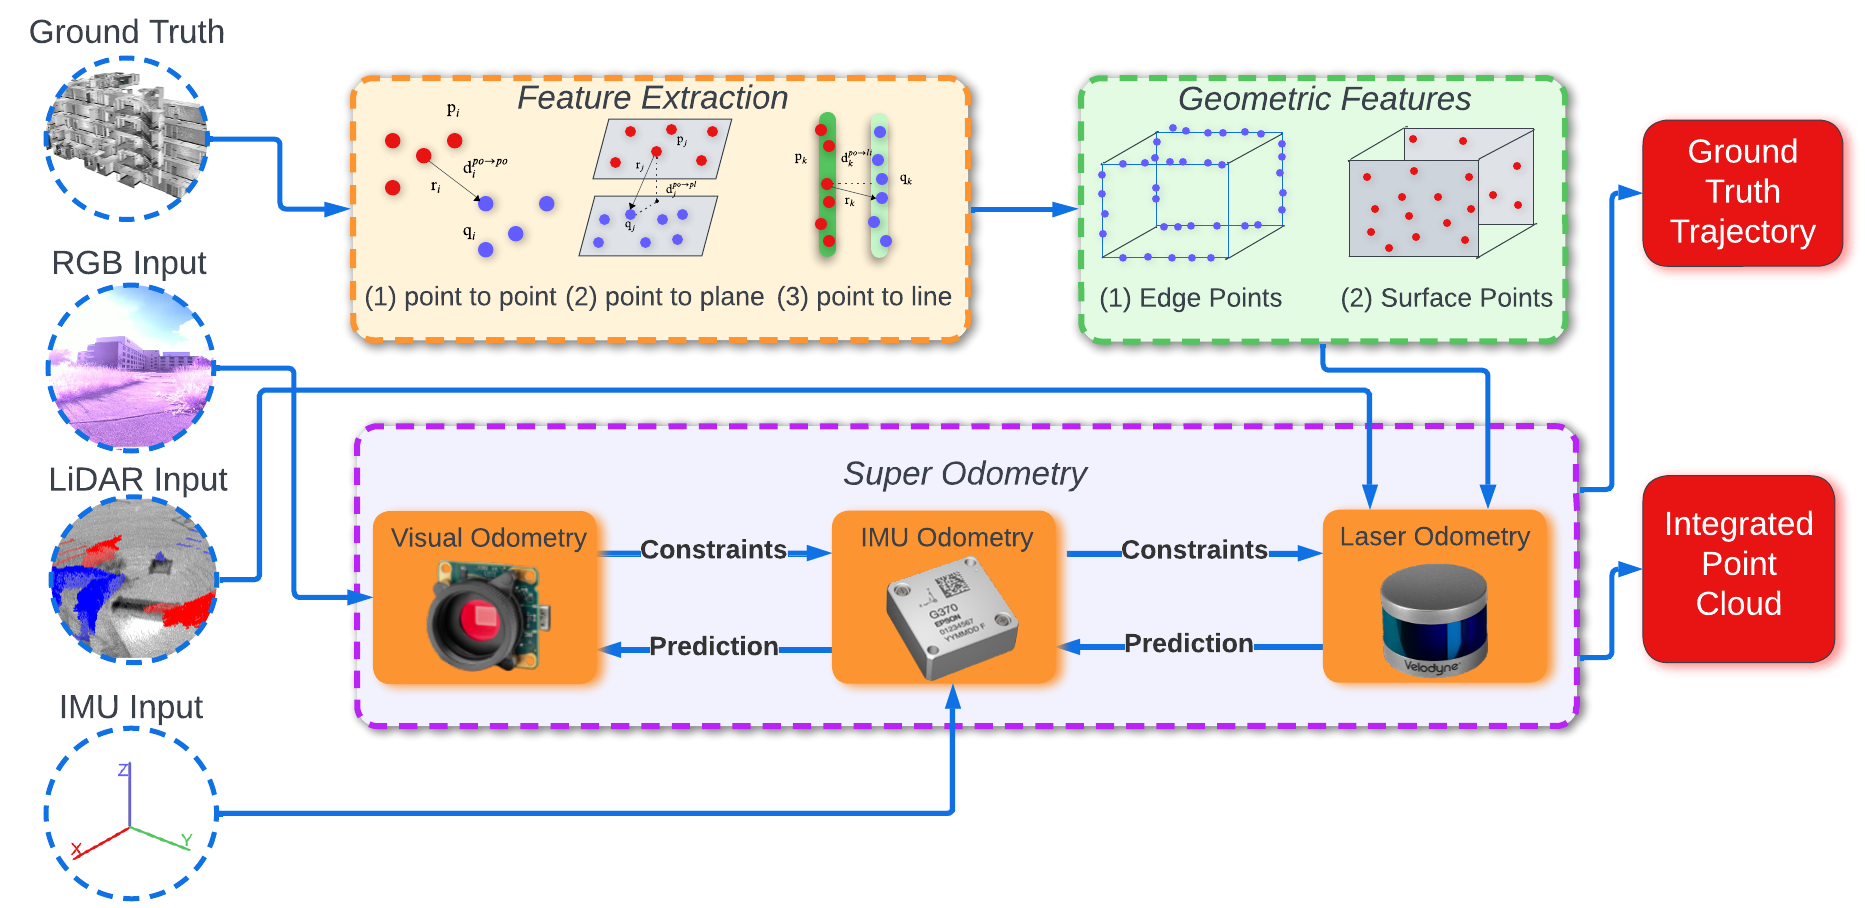
\includegraphics[width=0.9\textwidth,height=\textheight,keepaspectratio]{figure/localization_demo_10.png}
    \caption{Overview of ground truth trajectories generation on modified Super Odometry. Ground truth geometric features are extracted and stored in the pre-processing phase. Laser Odometry is modified to use stored ground truth features to provide accurate constraints. The ground truth trajectory is formed by collecting ground truth poses estimated by Super Odometry.}
    \label{fig:localization}
\end{figure*}

\begin{table*}
	\small
% 	\begin{center}
 \resizebox{\textwidth}{!}{
\begin{tabular}{ccc|cccccc}
\hline
\multicolumn{3}{c|}{Runs in Subt-MRS} & \multicolumn{6}{c}{SLAM Algorithms' Map Deviation (\%)}    \\
Robot &
  \multicolumn{1}{l}{Run Length (m)} &
  \multicolumn{1}{l|}{Run Time(s)} &
  \multicolumn{1}{l}{Fast\_LIO\cite{fastlio}} &
  \multicolumn{1}{l}{Faster\_LIO\cite{faster_lio}} &
  \multicolumn{1}{l}{LIO\_SAM\cite{liosam2020shan}} &
  \multicolumn{1}{l}{Clins\cite{clins}} &
  \multicolumn{1}{l}{ALOAM\cite{aloam}} &
  \multicolumn{1}{l}{Super Odometry\cite{zhao2021super}} \\ \hline
Canary      & 329        & 591.3      & $\ge$50  & 31.43 & $\ge$50 & 16.01 & 37.91 & \textbf{0.09}  \\
DS3         & 350.6      & 607.42     & 0.03     & 0.08  & $\ge$50 & 1.39  & 0.01  & \textbf{0.006} \\
DS4         & 238        & 484.7      & 13.78 & 12.48 & $\ge$50 & 3.43  & 10.72 & \textbf{0.15}  \\
R1          & 436.4      & 600        & 28.99 & 34.91 & $\ge$50 & 16.4  & 32.95 & \textbf{0.07}  \\
R2          & 536        & 1909       & 4.36  & 10.42 & $\ge$50 & 16.05 & 7.6   & \textbf{0.07}  \\
R3          & 642        & 1713       & $\ge$50    & $\ge$50 & $\ge$50 & $\ge$50  & 40.8  & \textbf{2.4}  
\end{tabular}
}
	\vspace{-0.1in}
% 	\end{center}
	\caption{Map Deviation of different SLAM algorithms running on Subt-MRS datasets}
	\vspace{-0.1in}
	\label{Tab:algorithm_compare}
\end{table*}

\section{Ground Truth Map}\label{sec:ground_truth}

\subsection{Instruments}
% \begin{figure*}[]
%   \centering
%   \begin{subfigure}{0.2\linewidth}
%     \centering
%     \includegraphics[scale=0.14]{figure/TS15.jpg}
%     \caption{Total Station}
%     \label{fig:TS}
%   \end{subfigure}
%   \hfill
%   \begin{subfigure}{0.2\linewidth}
%     \centering
%     \includegraphics[scale=0.55]{figure/mini360prism.jpg}
%     \caption{Leica Mini 360 Prism}
%     \label{fig:prism}
%   \end{subfigure}
%   \hfill
%   \begin{subfigure}{0.2\linewidth}
%     \centering
%     \includegraphics[scale=0.1]{figure/FARO.png}
%     \caption{FARO Scanner}
%     \label{fig:FARO}
%   \end{subfigure}
%   \hfill
%   \begin{subfigure}{0.2\linewidth}
%     \centering
%     \includegraphics[scale=0.25]{figure/faro-target.jpeg}
%     \caption{FARO Target}
%     \label{fig:target}
%   \end{subfigure}
%   \caption{Primary equipment used for ground truth data collection}
%   \label{fig:equipment}
% \end{figure*}

% \begin{figure}[bh!]
%   \centering
%   \begin{subfigure}[b]{0.18\textwidth}
%     \centering
%     \includegraphics[width=\textwidth]{figure/TS15.jpg}
%     \caption{Total Station}
%     \label{fig:TS}
%   \end{subfigure}
%   \hfill
%   \begin{subfigure}[b]{0.18\textwidth}
%     \centering
%     \includegraphics[width=\textwidth]{figure/mini360prism.jpg}
%     \caption{Leica Mini 360 Prism}
%     \label{fig:prism}
%   \end{subfigure}
%   \hfill
%   \begin{subfigure}[b]{0.18\textwidth}
%     \centering    \includegraphics[width=0.7\textwidth]{figure/FARO.png}
%     \caption{FARO Scanner}
%     \label{fig:FARO}
%   \end{subfigure}
%   \hfill
%   \begin{subfigure}[b]{0.18\textwidth}
%     \centering
%     \includegraphics[width=\textwidth]{figure/faro-target.jpeg}
%     \caption{FARO Target}
%     \label{fig:target}
%   \end{subfigure}
%   \caption{Primary equipment used for ground truth data collection}
%   \label{fig:equipment}
% \end{figure}
% In this section, we will introduce the equipments we used for getting a ground truth map.

% A Leica Viva Total Station 15A, shown in Figure \ref{fig:TS}, is a powerful survey laser rangefinder. It can measure distances to within 1 millimeter accuracy and angles to within 1 degree-second accuracy. It functions by sitting on a tripod and measuring the distance to either any object, such as a wall, or a small glass prism that provides very precise direct reflection for good range measurement. Such measurements can then be used after setting up the instrument in a different location, allowing the measurements from two positions to be placed in the same coordinate frame.

% A Leica Viva Total Station 15A, shown in Figure \ref{fig:TS} distances to within 1-millimeter accuracy and angles to within 3 degree-second accuracy. Multiple measurements made by the Total Station can be placed in the same coordinate frame later. Surveying techniques were used to generate site control points, create loop closure, and to gather measurements used to validate model data.

% A Leica Mini 360 Prism, shown in Figure \ref{fig:prism} is a glass prism with reflective backing on the inside oriented such that any reflection is parallel to the incident light. This is exploited by the Total Station, which emits a laser beam and measures its reflection. These prisms give the Total Station a very precise measurement target that can be seen from very long distances.


% A Leica Mini 360 Prism, shown in Figure \ref{fig:prism} is a precision glass reflector that parallelizes and returns the laser from the total station up to 350m to within 1.5-millimeter accuracy.  The robotic total station uses return signal to aim the instrument to the prism and records a horizontal angle, vertical angle, and distance to the prism during each measurement.  Robotic aiming provides consistent, accurate, and reliable measurements and was particularly useful for this application in the unlit hallways and interior spaces modeled.  

% A FARO Focus 3D S120, shown in Figure \ref{fig:FARO}, is a very precise point cloud measurement tool. It sits on a tripod and slowly rotates while a mirror rotates very fast while a laser points at it. It reads the reflection of each flash of the laser beam, creating a dense point cloud. It is capable of measuring 100,000-1,000,000 points/second. Its range accuracy can be between 0.3mm and 2.2mm depending on the environment, range, and whether or not multi-point averaging is used. Its angular step size is 0.009 degrees.

% A FARO Focus 3D S120, shown in Figure \ref{fig:FARO}, is a precise dense point cloud measurement tool. The tripod mounted scanner has a laser ranger that hits a spinning mirror sweeping a vertical plane while being rotated to obtain 360° horizontal and 300° vertical spherical measurements to surfaces.   The angular step size is 0.009 degrees and Its range accuracy is between 0.3mm and 2.2mm, depending on the environment, range, and whether multi-point averaging is used.  Typical scan settings for this project were Resolution ¼, Quality 3X, and no color data with each scan taking 5 minutes and gathering 43.7 million points with an accuracy of 6.1mm at 10 meters.  Matching and alignment of scans was conducted using Autodesk Recap Pro and Cloud Compare software.  To supplement matching and alignment checkerboard fiducial targets were used in select areas.  The target shown in Figure \ref{fig:target} provide different reflectivity intensities measured by the FARO Scanner and the post processing software has integrated target recognition elements that precisely locate the target intersection.

% This section introduces the equipment used for creating a ground truth map. The Leica Viva Total Station 15A was used for distance and angle measurements with high accuracy. The Total Station allowed multiple measurements to be placed in the same coordinate frame for later use. Surveying techniques were used to generate site control points, create loop closure, and validate model data.

% The Leica Mini 360 Prism is a precision glass reflector that returns the laser from the Total Station with high accuracy up to 350m. The robotic total station records a horizontal angle, vertical angle, and distance to the prism during each measurement. Robotic aiming provided consistent, accurate, and reliable measurements, which were particularly useful in unlit hallways and interior spaces.

% The FARO Focus 3D S120 is a precise dense point cloud measurement tool that uses a laser ranger to obtain 360° horizontal and 300° vertical spherical measurements to surfaces. The scanner has high accuracy, with a range accuracy between 0.3mm and 2.2mm, depending on the environment and range. Typical scan settings for this project were Resolution ¼, Quality 3X, and no color data. Matching and alignment of scans were conducted using Autodesk Recap Pro and Cloud Compare software, with checkerboard fiducial targets used in select areas to supplement matching and alignment. The post-processing software integrated target recognition elements that precisely located the target intersection.
In our approach to creating a ground truth map, we utilize a combination of surveying techniques and advanced measurement tools. Specifically, the Leica Viva Total Station 15A is used to provide accurate distance and angle measurements. The Leica Mini 360 Prism is utilized to reflect the laser back to the Total Station with high precision, and the robotic aiming feature is employed to ensure consistency and reliability in unlit hallways and interior spaces. Additionally, we use the FARO Focus 3D S120 for precise dense point cloud measurements, with its high accuracy obtained through a laser ranger. Finally, checkerboard fiducial targets are used in select areas to supplement the software used for matching and alignment.
\subsection{Data Collection}



This study performs Ground Truth modeling at two locations in Pittsburgh, PA, USA: an abandoned hospital and Carnegie Mellon University campus. The hospital survey utilizes a Total Station survey instrument with eye bolts installed at strategic locations to measure points around a large loop. With the loop closure algorithm, an error of approximately 3.4 cm is yielded, and the model covers an area of roughly 350 meters by 350 meters, including several buildings and surrounding landscapes. 
% (See Figure \ref{fig:dc1} for the model generated from this survey.)
On the other hand, the Carnegie Mellon University campus survey focuses on four buildings near the Newell-Simon Hall and utilizes 79 FARO scans to generate a model with an expected accuracy of less than 2cm. The survey covers an area of about 200 meters by 200 meters and results in a highly accurate model 
% (See Figure \ref{fig:dc2} for the model generated from this survey.)
The dataset generated from these surveys exceeds 750Gb of data, providing valuable resources for various research and applications. The ground truth maps for all the datasets will be provided to the users. A glimpse of these ground truth maps is provided in the supplementary material.

% At both sites, the FARO laser scanner was used to take several hundred scans, with seven including FARO checkerboard targets. The resulting dataset covered approximately 550 square meters and had less than 2cm accuracy. To create the models, raw scans were integrated into large high-density models using Recap Pro software, with points averaged to 20mm density and saved as Cloud Compare .bin files. The model matching projected over the large sites is expected to be better than 50cm. The generated dataset, exceeding 750Gb of data, is highly accurate and comprehensive, making it a valuable resource for a wide range of research and applications.

\subsection{Ground Truth Trajectory}
\subsubsection{Generation}
Ground truth trajectories are generated for all datasets, using Super Odometry \cite{zhao2021super} with a modified Laser Odometry algorithm. As shown in Figure \ref{fig:localization}, the ground truth point cloud is pre-processed using a feature extraction module that assesses ``local linearity, planarity, and curvatures of geometric feature'' \cite{zhao2021super}, with the extracted geometric features stored. As new LiDAR scans arrive, a subset of the ground truth points is selected from the stored features based on the current pose and used as the reference for Iterative Closest Point (ICP). The resulting ICP output is integrated into the normal Super Odometry procedures. Visual Odometry is employed to help constrain pose estimation in datasets with degraded geometry, such as long corridor environments.

% \begin{figure}[ht!]
%     \includegraphics[width=\linewidth]{figure/long_corridor_analysis.png}
%     \caption{The evaluation result of one generated trajectory for long corridor environment. Green points represent inliers and red points represent outliers}
%     \label{fig:long_corridor_analysis}
% \end{figure}
\subsubsection{Evaluation}
 In this study, we assess the accuracy of the created trajectories by employing Map Analysis\footnote{\href{https://github.com/subtchallenge/map_analysis}{https://github.com/subtchallenge/map\_analysis}}, an open-source tool that calculates the map deviation utilizing both the integrated point cloud and the ground truth map. The modified ground truth trajectories provide both the trajectory and the integrated point cloud. To quantify the map deviation, we introduce the distance metric $d_{i}^{j}$, defined as the euclidean distance between point $i$ and its corresponding point $j$ in the ground truth map. We then identify the set of outlier points using the deviation threshold of $1.0m$ specified in Equation \ref{eq:outlier_points}.
\begin{equation}\label{eq:outlier_points}
\mathrm{Outlier\,Points:} d_{i}^{j} > 1.0m
\end{equation}
The map deviation is computed by dividing the number of outlier points by the total number of points, as shown in Equation \ref{eq:map_deviation}. 
\begin{equation}\label{eq:map_deviation}
\sigma = \frac{N_{\mathrm{Outlier\,Points}}}{N_{\mathrm{Total\,Points}}}
\end{equation}
To ensure the validity of the generated ground truth trajectory, we require that the map deviation of its integrated point cloud is less than $1\%$. This threshold value accounts for the possibility that some LiDAR scan points may not be covered by the ground truth map. Notably, we observe that all the identified outliers originate from rooms that lie outside the coverage area of the ground truth map for the long corridor. After excluding the points in the rooms outside the coverage area of the ground truth map for the long corridor, our trajectory generation result achieved a map deviation of less than $0.1\%$.
% \begin{figure*}[]
%   \begin{subfigure}{0.25\linewidth}
%     \centering
%     \includegraphics[scale=0.25]{figure/Groundtruth_p3.png}
%     \caption{Long corridors are challenging due to low features}
%     \label{fig:corridors}
%   \end{subfigure}
%   \hfill
%   \begin{subfigure}{0.35\linewidth}
%     \centering
%     \includegraphics[scale=0.25]{figure/Groundtruth_p2.png}
%     \caption{Winding staircases are challenging for SLAM environments}
%     \label{fig:staircases}
%   \end{subfigure}
%   \hfill
%   \caption{Complex and challenging geometrically degraded environments of the collected data set enable rigorous testing of SLAM environments and place recognition algorithms. }
% \end{figure*}


% \subsubsection{Ground Truth Trajectory Generation}
% it depends if we have enough time to finish it (probably will skip it)

% \subsubsection{Accuracy Metric}

% \subsubsection{Robustness Metric}


\section{Challenging Results and Findings}\label{sec:results}

\subsection{Results}

% The Subt-MRS dataset serves as a rigorous benchmark for assessing the robustness of the current state-of-the-art SLAM algorithms. In order to gain insight into the limitations of these methods, we conduct evaluations on several LiDAR-only, LiDAR-Inertial, and LiDAR-Visual-Intertial SLAM algorithms across different runs in our dataset. We select three runs collected by drones (Canary, DS3, DS4) and three runs collected by ground robots (R1, R2, R3) in a distinct section of the subterranean environment. The point cloud data is depicted in Figure \ref{fig:subt_pointcloud}. We particularly focus on R3's LiDAR, which exhibits a significantly higher level of sensor noise, and collect sequences from this robot to assess the robustness of the algorithms under the disturbance in LiDAR measurements. Finally, we compare the reconstructed maps against the ground truth map to estimate the map deviations. The results of the map deviation analysis for each algorithm on data collected by different robots in our dataset are presented in Table \ref{Tab:algorithm_compare}.
The Subt-MRS dataset provides a comprehensive framework for evaluating the performance of different SLAM algorithms. To analyze the limitations of current state-of-the-art SLAM methods, we conduct extensive evaluations on various LiDAR-only, LiDAR-Inertial, and LiDAR-Visual-Intertial SLAM algorithms using our dataset. To ensure diversity in our analysis, we select three runs collected by drones (Canary, DS3, DS4) and three runs collected by ground robots (R1, R2, R3) in a distinct section of the subterranean environment. In our evaluations, we focus on the LiDAR data from R3, which has a higher level of sensor noise and collect sequences to assess the algorithms' robustness under such disturbances. To quantify the performance of each algorithm, we compare the reconstructed maps against the ground truth map and estimate the map deviations. Our results are presented in Table \ref{Tab:algorithm_compare}, and the point cloud data used in our evaluations are shown in Figure \ref{fig:subt_pointcloud}.

\subsection{Discussion}
% Based on the results in Table \ref{Tab:algorithm_compare}, we observe that, with the exception of LIO\_SAM, all the algorithms achieve map deviations of less than $50\%$ in most runs. Super Odometry \cite{zhao2021super}, which utilizes LiDAR, visual camera, and IMU, achieves the lowest deviation of $0.5\%$ on average, indicating the highest degree of robustness among all the algorithms. The visual sensor component in Super Odometry provides additional resilience in the face of the challenging environmental conditions present in our dataset. In particular, Super Odometry performs well, with only $2.4\%$ deviation, in the run collected by R3, which exhibits high noise levels in the LiDAR measurements. The remaining algorithms show deviations of greater than $40\%$ in R3. Among the other algorithms, Clins \cite{clins} achieves the lowest deviation ($\leq 17\%$) in most runs. Clins operates offline and implements continuous-time trajectory estimation, which results in better performance over other LiDAR-Inertial and LiDAR-Only algorithms. Conversely, Fast\_LIO \cite{fastlio}, Faster\_LIO \cite{faster_lio}, and ALOAM \cite{aloam} show significant drift in most runs. In general, most LiDAR-Inertial and LiDAR-Only SLAM algorithms demonstrate limited capacity to achieve high robustness in multi-degraded environments. 
The evaluation results in Table \ref{Tab:algorithm_compare} provide insights into the performance of various SLAM algorithms on the Subt-MRS dataset. Super Odometry stands out as the most robust algorithm, achieving an average deviation of only $0.5\%$. The combination of LiDAR, visual camera, and IMU sensors in Super Odometry provides greater resilience against challenging environmental conditions. In contrast, LiDAR-Inertial and LiDAR-Only algorithms, such as Fast\_LIO, Faster\_LIO, and ALOAM, show significant drift in most runs, indicating limited robustness in multi-degraded environments. Clins, which implements continuous-time trajectory estimation, performs better than other LiDAR-Inertial and LiDAR-Only algorithms, with deviations of less than $17\%$ in most runs. However, Clins operates offline, which may not be suitable for real-time applications. The results suggest that the use of additional sensors and advanced estimation techniques is necessary to achieve high robustness in challenging environments.


%------------------------------------------------------------------------

{\small
\bibliographystyle{ieee_fullname}
\bibliography{egbib}
}

% \newpage
% \appendix
% \twocolumn[\centering \section*{SubT-MRS: A Subterranean, Multi-Robot, Multi-Spectral and\\Multi-Degraded Dataset for Robust SLAM \\ [1.3ex]Supplementary Material}]


% \section{Overview}

% In this supplementary material, we will focus specifically on discussing the extrinsic calibration between robots and providing more details about our dataset. We will dive into the metrics we used to evaluate the difficulty of our dataset and provide a thorough analysis of the results. Finally, we will also provide the ground truth 3D models of other environments for reference and comparison.

% \section{Extrinsic Calibration Between Robots}

% The extrinsic map calibration procedure for multiple robots was explained briefly in the context of Generalized-ICP (GICP) in the paper. Specifically, we developed the "Auto Extrinsic Calibration" algorithm, as shown in Figure~\ref{fig:robot_extrinsic_cal}, which we will explain in detail in this section.

% \begin{itemize}
%     \item Step1: a lead robot is taken to the calibration position and it creates a local point cloud map of its surroundings. This map is then shared with the base station and obtain the transformation $T^d_{m_0} = {\mathbf{R}, \mathbf{t} }$. This is the reference map that other robots will use to calibrate. The lead robot is then moved from the calibration position to make way for other robots.
    
%     \item Step2: subsequent robots are taken to the calibration position to create a local map of their surrounding, and shares its pose with respect to its own map frame $T^{m_0}_{b_0}$. All subsequent robots are placed in the same position, receive reference information from the base station, and use Generalized Iterative Closest Point (GICP) \cite{segal2009generalized} to align their current keyframes $P_i$ to $P_0$, obtaining $T^{b_0}_{b_i}$.
% \end{itemize}

% Finally, for each robot $i$, we obtain the solution:

% \begin{equation}
% T^d_{m_i} = T^d_{m_0} T^{m_0}_{b_0} T^{b_0}_{b_i} (T^{m_i}_{b_i})^{-1}
% \end{equation}


% This method ensures effective collaboration between the robots by ensuring that they all operate in the same spatial orientation, enabling them to complete the task with precision and accuracy. A visual description of this procedure is provided in Fig \ref{fig:robot_extrinsic_cal}.










% % Collaborative tasks require multiple robots to operate in a common frame of reference. Our procedure to create this involves the usage of Generalized-ICP (GICP)\cite{segal2009generalized} and is two-fold. In the first step, one robot shares its map from a feature-rich location to a base station. In the second step, the remaining robots take turns solving a GICP, in the same feature-rich location as the first robot and obtain a frame transformation from its own to the first robot. All the robots end up in a common frame after this procedure and build their map further using Super Odometry\cite{zhao2021super}. We will provide a graphic and mathematical description of this process in the supplemental material.


% % In the first step, a lead robot is taken to the calibration position and it creates a local point cloud map of its surroundings. This map is then shared with the base station. This is the reference map that other robots will use to calibrate. The lead robot is then moved from the calibration position to make way for other robots. 

% % In the second step, subsequent robots are taken to the calibration position to create a local map of their surrounding. The reference map is shared from the base station with the robot. A GICP registration between the reference map and the local map of the robot is computed. This transformation is used to align the map of this robot to the reference map. After registration, the robot is moved from the calibration position, and the steps are repeated for the remaining robots

% % This method ensures effective collaboration between the robots by ensuring that they all operate in the same spatial orientation, enabling them to complete the task with precision and accuracy. A visual description of this procedure is provided in Fig 
% % \ref{fig:autocalib}


% % To finish a collaborative task, multiple robots need to operate in a common frame of reference. This is achieved by computing the relative rigid-body transformation of the robots with respect to a pre-specified reference frame. We achieve this using a procedure called Auto Calibration (AC), based on Generalized-ICP (GICP) \cite{segal2009generalized}. The AC procedure has two steps. In the first step, a lead robot moves to the calibration position and captures its surroundings with the point cloud, after which, it shares this map with the base station. In the second step, each subsequent robot is taken to the calibration position. It captures its local map and requests the reference map from the base station. Finally, a GICP registration between the reference map and the local map is computed. This result will align each robot with the reference frame created by the first robot. Once complete, the robot moves from this position and the steps are repeated for the remaining robots. A description of the information flow is given in Fig \ref{fig:autocalib}.


% \begin{figure*}[h!]
%     \centering
%     \includegraphics[width=0.9\textwidth, height=0.9\textheight, keepaspectratio]{figure/autocal_new.png}
%     \caption{Extrinsic Calibration between robots.  At least one robot shares its local map to the basestation. Subsequent robots may request this map from the basestation and perform alignment with respect to its own local map}
%     \label{fig:robot_extrinsic_cal}
% \end{figure*}




% \section{Datasets List}
% We have statistically analyzed some of our datasets and provided the results in Tables \ref{tab:dataset_descrip}-\ref{tab:dataset_sensors}. There are a total of 9 single-robot datasets that have been analyzed. Table \ref{tab:dataset_descrip} gives a detailed description of the datasets we have collected. This table has been split into 9 columns which provide information like the environment type, vehicle type, dataset difficulty, ground truth information, etc.  The first 6 datasets starting with the name ``SubT'' are datasets collected from the final challenge of the DARPA Subterranean Challenge and feature mostly underground data. The last 3 datasets starting with the name ``Hawkins'' have been collected at an abandoned hospital building and feature indoor-outdoor as well as multi-floor datasets. Table \ref{tab:dataset_degradation} lists down the type of degradations present in each dataset listed in Table \ref{tab:dataset_descrip}. Table \ref{tab:dataset_sensors} lists down the sensors used in the datasets listed in Table \ref{tab:dataset_descrip}. These datasets are only a minor part of our dataset collection and more dataset is being prepared and analyzed. Final dataset including runs with all four sensors namely, IMU, LiDAR, RGB camera, and thermal camera, multi-robot runs, and runs in the university campus, caves, and tunnels will be released upon article acceptance.




% \begin{table*}[h!]
% \centering
% \caption{Detailed dataset information}
% \label{tab:dataset_descrip}
% \begin{tabular}{|c||c|c|c|c|c|c|c|c|} 
% \hline
% \textbf{Dataset Name} & \begin{tabular}[c]{@{}c@{}}\textbf{Environment}\\\textbf{Type}\end{tabular} & \begin{tabular}[c]{@{}c@{}}\textbf{Vehicle~}\\\textbf{Type}\end{tabular} & \begin{tabular}[c]{@{}c@{}}\textbf{Max~}\\\textbf{Speed}\\\textbf{(m/s)}\end{tabular} & \begin{tabular}[c]{@{}c@{}}\textbf{Motion }\\\textbf{ Type}\end{tabular} & \begin{tabular}[c]{@{}c@{}}\textbf{Trajectory }\\\textbf{ Length(m)}\end{tabular} & \textbf{\textbf{Difficulty}} & \begin{tabular}[c]{@{}c@{}}\textbf{GT Map }\\\textbf{ Available}\end{tabular} & \begin{tabular}[c]{@{}c@{}}\textbf{GT Trajectory}\\\textbf{ Available}\end{tabular} \\ 
% \hline
% SubT Canary & Underground & UAV & 2 & Flying & 282.69 & High & YES & YES \\ 
% \hline
% SubT DS3 & Underground & UAV & 2 & Flying & 332.26 & Medium & YES & YES \\ 
% \hline
% SubT DS4 & Underground & UAV & 2 & Flying & 268.36 & Medium & YES & YES \\ 
% \hline
% SubT R1 & Underground & UGV & 4 & Roving & 203.3 & Low & YES & YES \\ 
% \hline
% SubT R2 & Underground & UGV & 4 & Roving & 536 & High & YES & YES \\ 
% \hline
% SubT R3 & Underground & UGV & 4 & Roving & 593.79 & High & YES & YES \\ 
% \hline
% \begin{tabular}[c]{@{}c@{}}Hawkins\\Long Corridor1\end{tabular} & Indoors & UGV & 6 & Roving & 616.45 & High & YES & YES \\ 
% \hline
% \begin{tabular}[c]{@{}c@{}}Hawkins\\Long Corridor2\end{tabular} & Indoors & UGV & 6 & Roving & 765 & High & YES & YES \\ 
% \hline
% \begin{tabular}[c]{@{}c@{}}Hawkins\\Multi-floor\end{tabular} & \begin{tabular}[c]{@{}c@{}}Indoors, \\multi-floor\end{tabular} & \begin{tabular}[c]{@{}c@{}}Legged\\Robot\end{tabular} & 1.5 & Walking & 270 & High & YES & YES \\
% \hline
% \end{tabular}
% \end{table*}


% \begin{table*}[h!]
% \centering
% \caption{Perceptual degradations present in the datasets}
% \label{tab:dataset_degradation}
% \begin{tabular}{|c||c|c|c|c|c|c|} 
% \hline
% \textbf{Dataset Name} & \textbf{Smoke} & \textbf{Dust} & \textbf{Low Illumination} & \textbf{Long Corridor} & \textbf{\textbf{Stairs}} & \textbf{Fast Rotations} \\ 
% \hline
% SubT Canary & \cmark  &  \cmark & \cmark  & \cmark & \xmark  &\cmark  \\ 
% \hline
% SubT DS3 & \cmark &  \cmark & \cmark & \cmark &\cmark  & \cmark \\ 
% \hline
% SubT DS4 &  \cmark &  \cmark & \cmark & \cmark &\cmark  & \cmark  \\ 
% \hline
% SubT R1 & \cmark & \xmark & \cmark  & \cmark  & \xmark  & \xmark  \\ 
% \hline
% SubT R2 & \cmark & \xmark & \cmark  & \cmark  & \xmark  & \xmark\\ 
% \hline
% SubT R3 & \cmark & \xmark & \cmark  & \cmark  & \xmark  & \xmark  \\
% \hline
% \begin{tabular}[c]{@{}c@{}}Hawkins\\Long Corridor1\end{tabular} & \xmark & \xmark  & \cmark & \cmark & \xmark & \cmark  \\ 
% \hline
% \begin{tabular}[c]{@{}c@{}}Hawkins\\Long Corridor2\end{tabular} &\xmark & \xmark  & \cmark & \cmark & \xmark & \cmark \\ 
% \hline
% \begin{tabular}[c]{@{}c@{}}Hawkins\\Multi-floor\end{tabular} & \xmark & \xmark  & \cmark  & \xmark  & \cmark & \xmark  \\
% \hline
% \end{tabular}
% \end{table*}

% \begin{table*}[h!]
% \centering
% \caption{Sensors used in the datasets}
% \label{tab:dataset_sensors}
% \begin{tabular}{|c||c|c|c|} 
% \hline
% \textbf{Dataset Name} & \textbf{IMU} & \textbf{LiDAR} & \textbf{RGB Camera} \\ 
% \hline
% SubT Canary & \cmark & \cmark & \xmark  \\ 
% \hline
% SubT DS3 &\cmark & \cmark & \xmark  \\ 
% \hline
% SubT DS4 &\cmark & \cmark & \xmark  \\ 
% \hline
% SubT R1 &\cmark & \cmark & \xmark  \\ 
% \hline
% SubT R2 &\cmark & \cmark & \xmark  \\ 
% \hline
% SubT R3 &\cmark & \cmark & \xmark  \\ 
% \hline
% \begin{tabular}[c]{@{}c@{}}Hawkins\\Long Corridor1\end{tabular}  & \cmark  & \cmark & \cmark \\ 
% \hline
% \begin{tabular}[c]{@{}c@{}}Hawkins\\Long Corridor2\end{tabular} & \cmark  & \cmark & \cmark \\ 
% \hline
% \begin{tabular}[c]{@{}c@{}}Hawkins\\Multi-floor\end{tabular} &  \cmark  & \cmark & \cmark \\ 
% \hline
% \end{tabular}
% \end{table*}

% \section{Datasets Evaluation}
% % Subt Env
% \begin{figure*}[ht!]
%     \centering
%     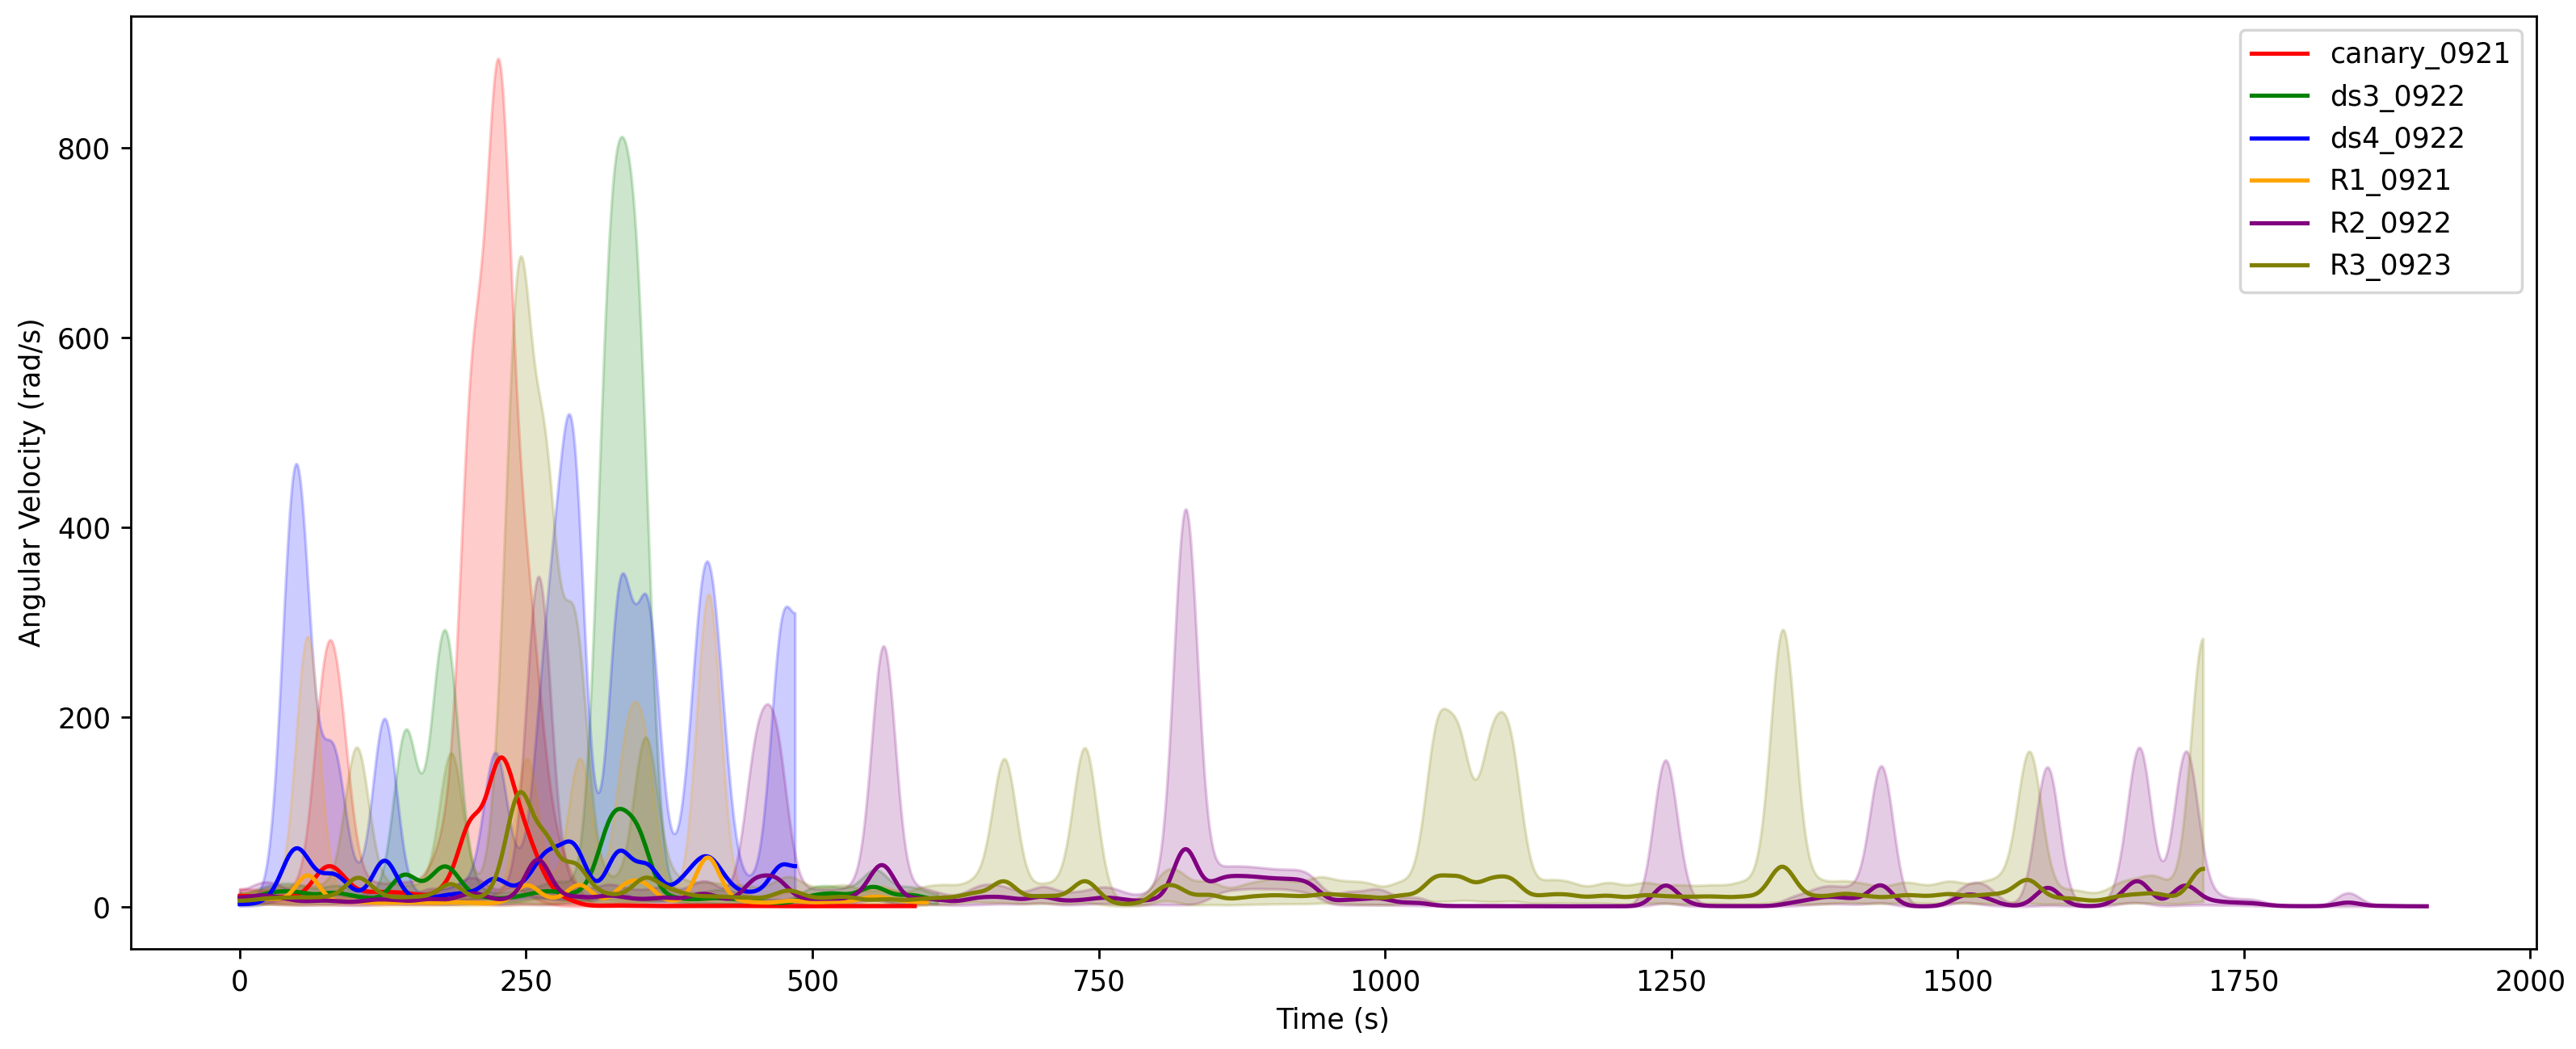
\includegraphics[width=0.9\textwidth,keepaspectratio]{figure/subt_angular.png}
%     \caption{The angular rate versus time graph for all runs collected in the SubT environment.}
%     \label{fig:subt_angular}
% \end{figure*}
% \begin{figure*}[ht!]
%     \centering
%     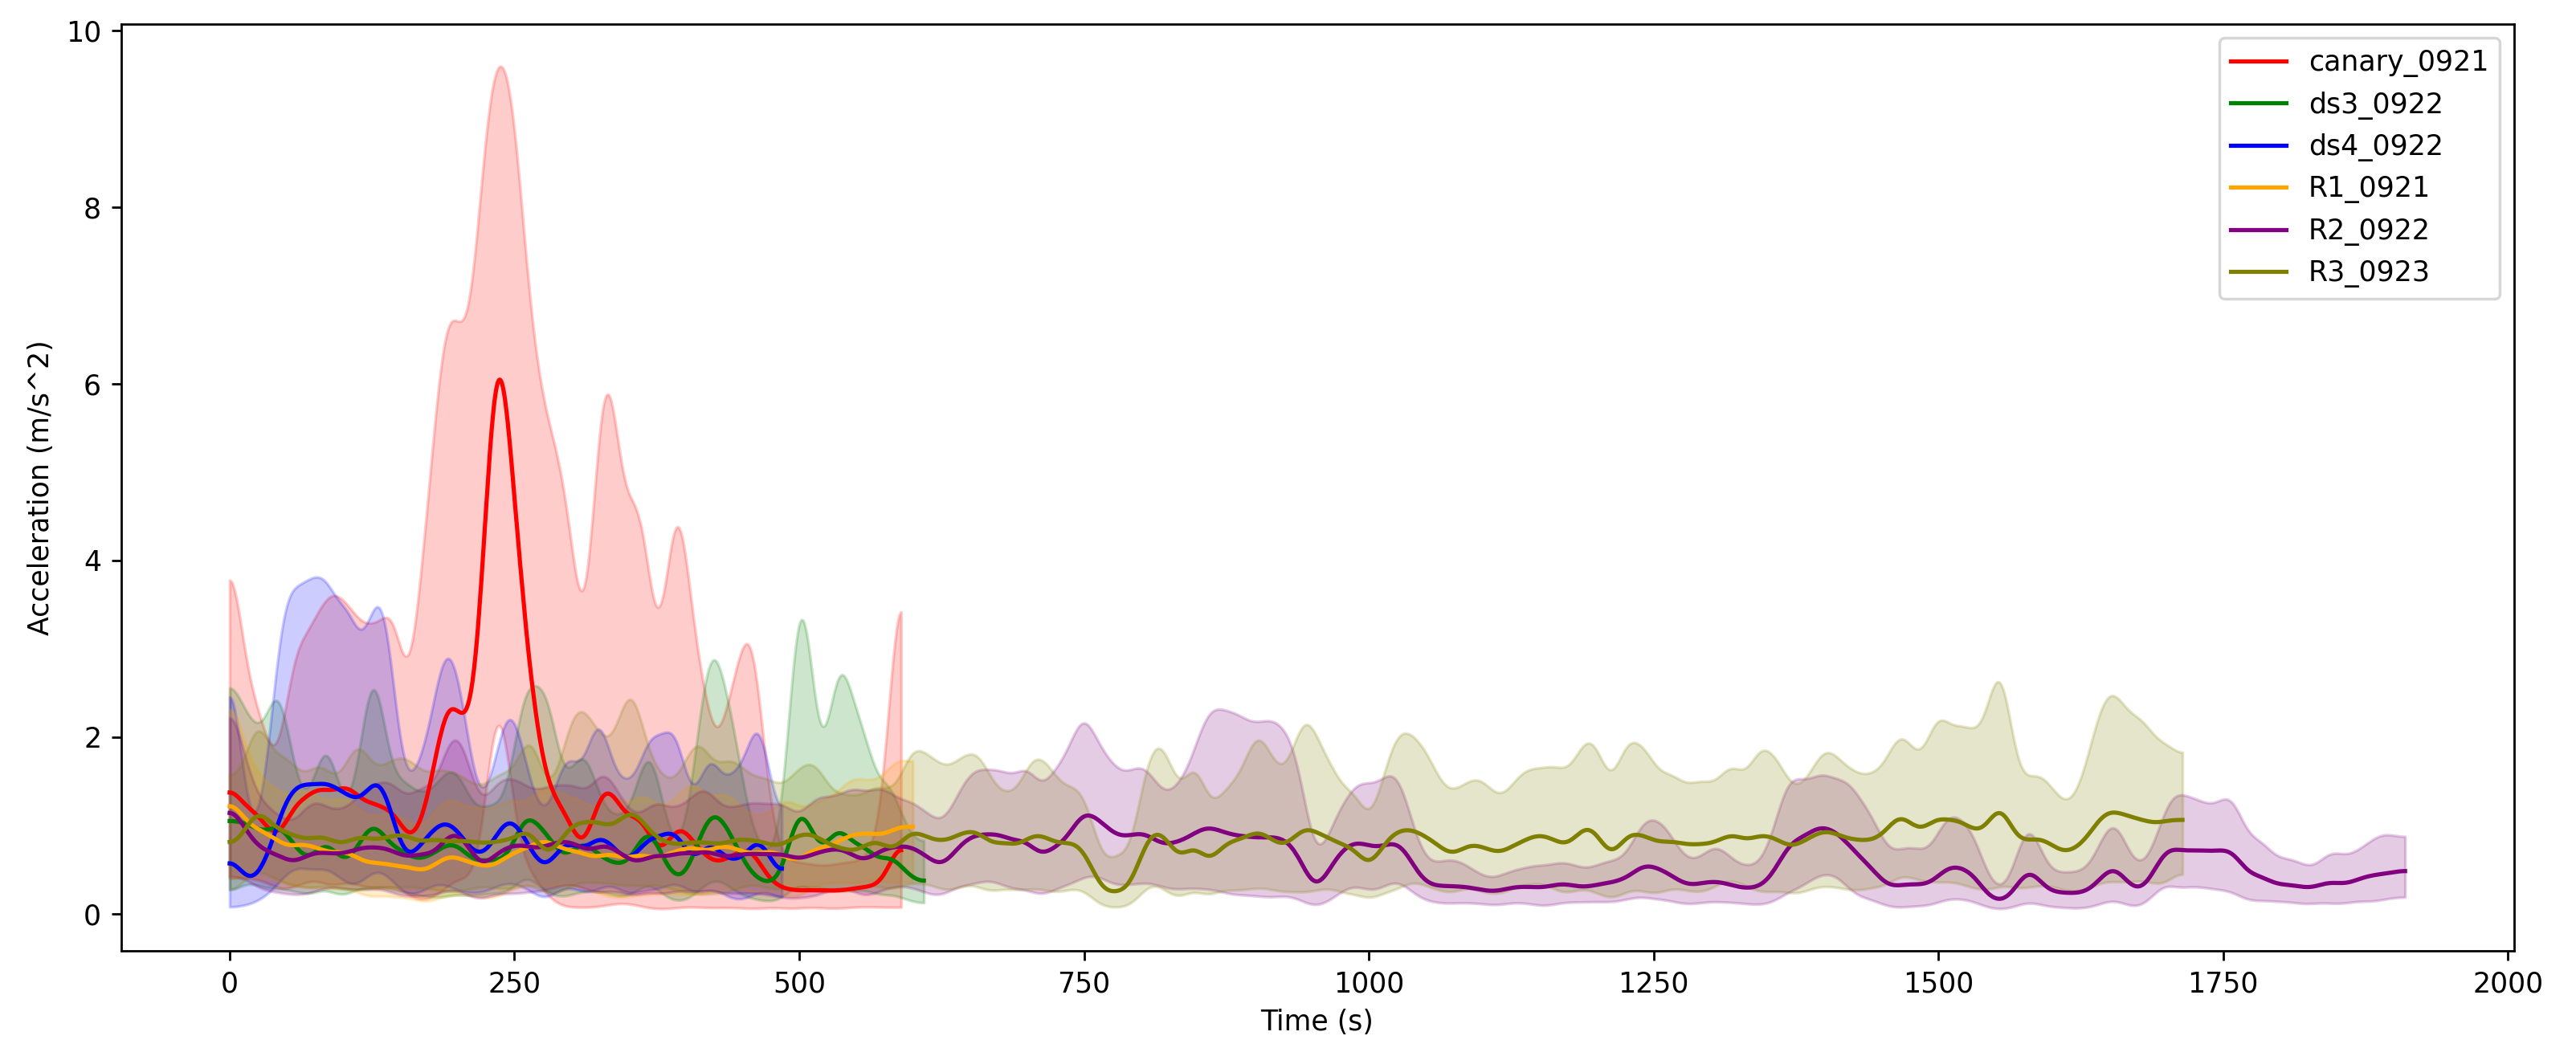
\includegraphics[width=0.9\textwidth,keepaspectratio]{figure/subt_accel.png}
%     \caption{The acceleration versus time graphs for all runs collected in the SubT environment. It can be seen that the SubT Canary dataset has the highest accelerations of all the datasets, which induces challenge for SLAM}
%     \label{fig:subt_accel}
% \end{figure*}
% \begin{figure*}[ht!]
%     \centering
%     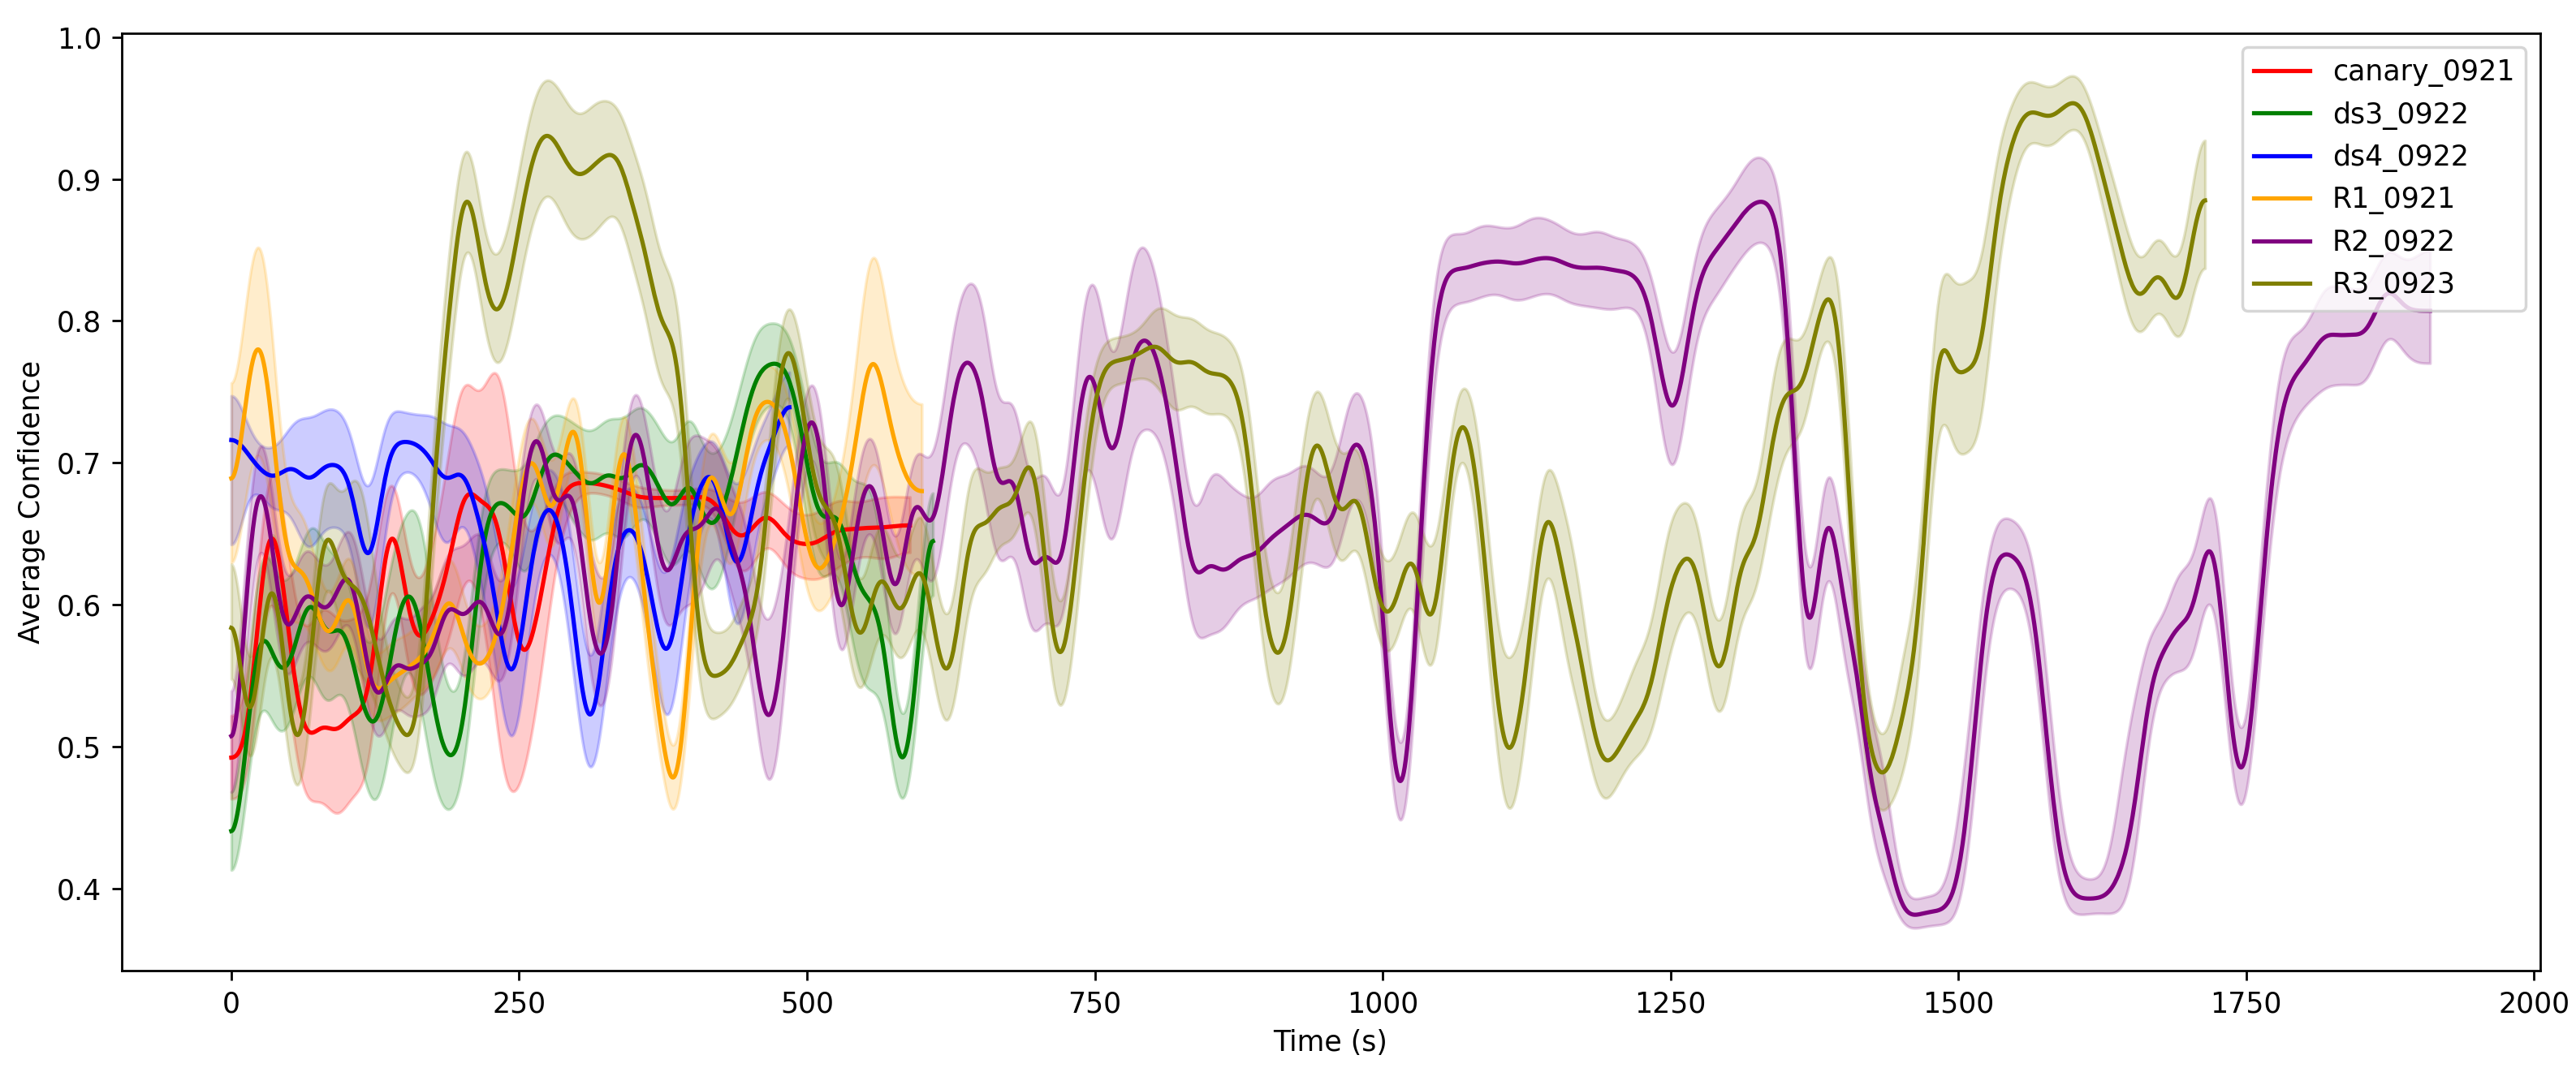
\includegraphics[width=0.9\textwidth,keepaspectratio]{figure/subt_confidence.png}
%     \caption{The confidence versus time graphs for all runs collected in the SubT environment.}
%     \label{fig:subt_confidence}
% \end{figure*}

% % Hawkins Env
% \begin{figure*}[ht!]
%     \centering
%     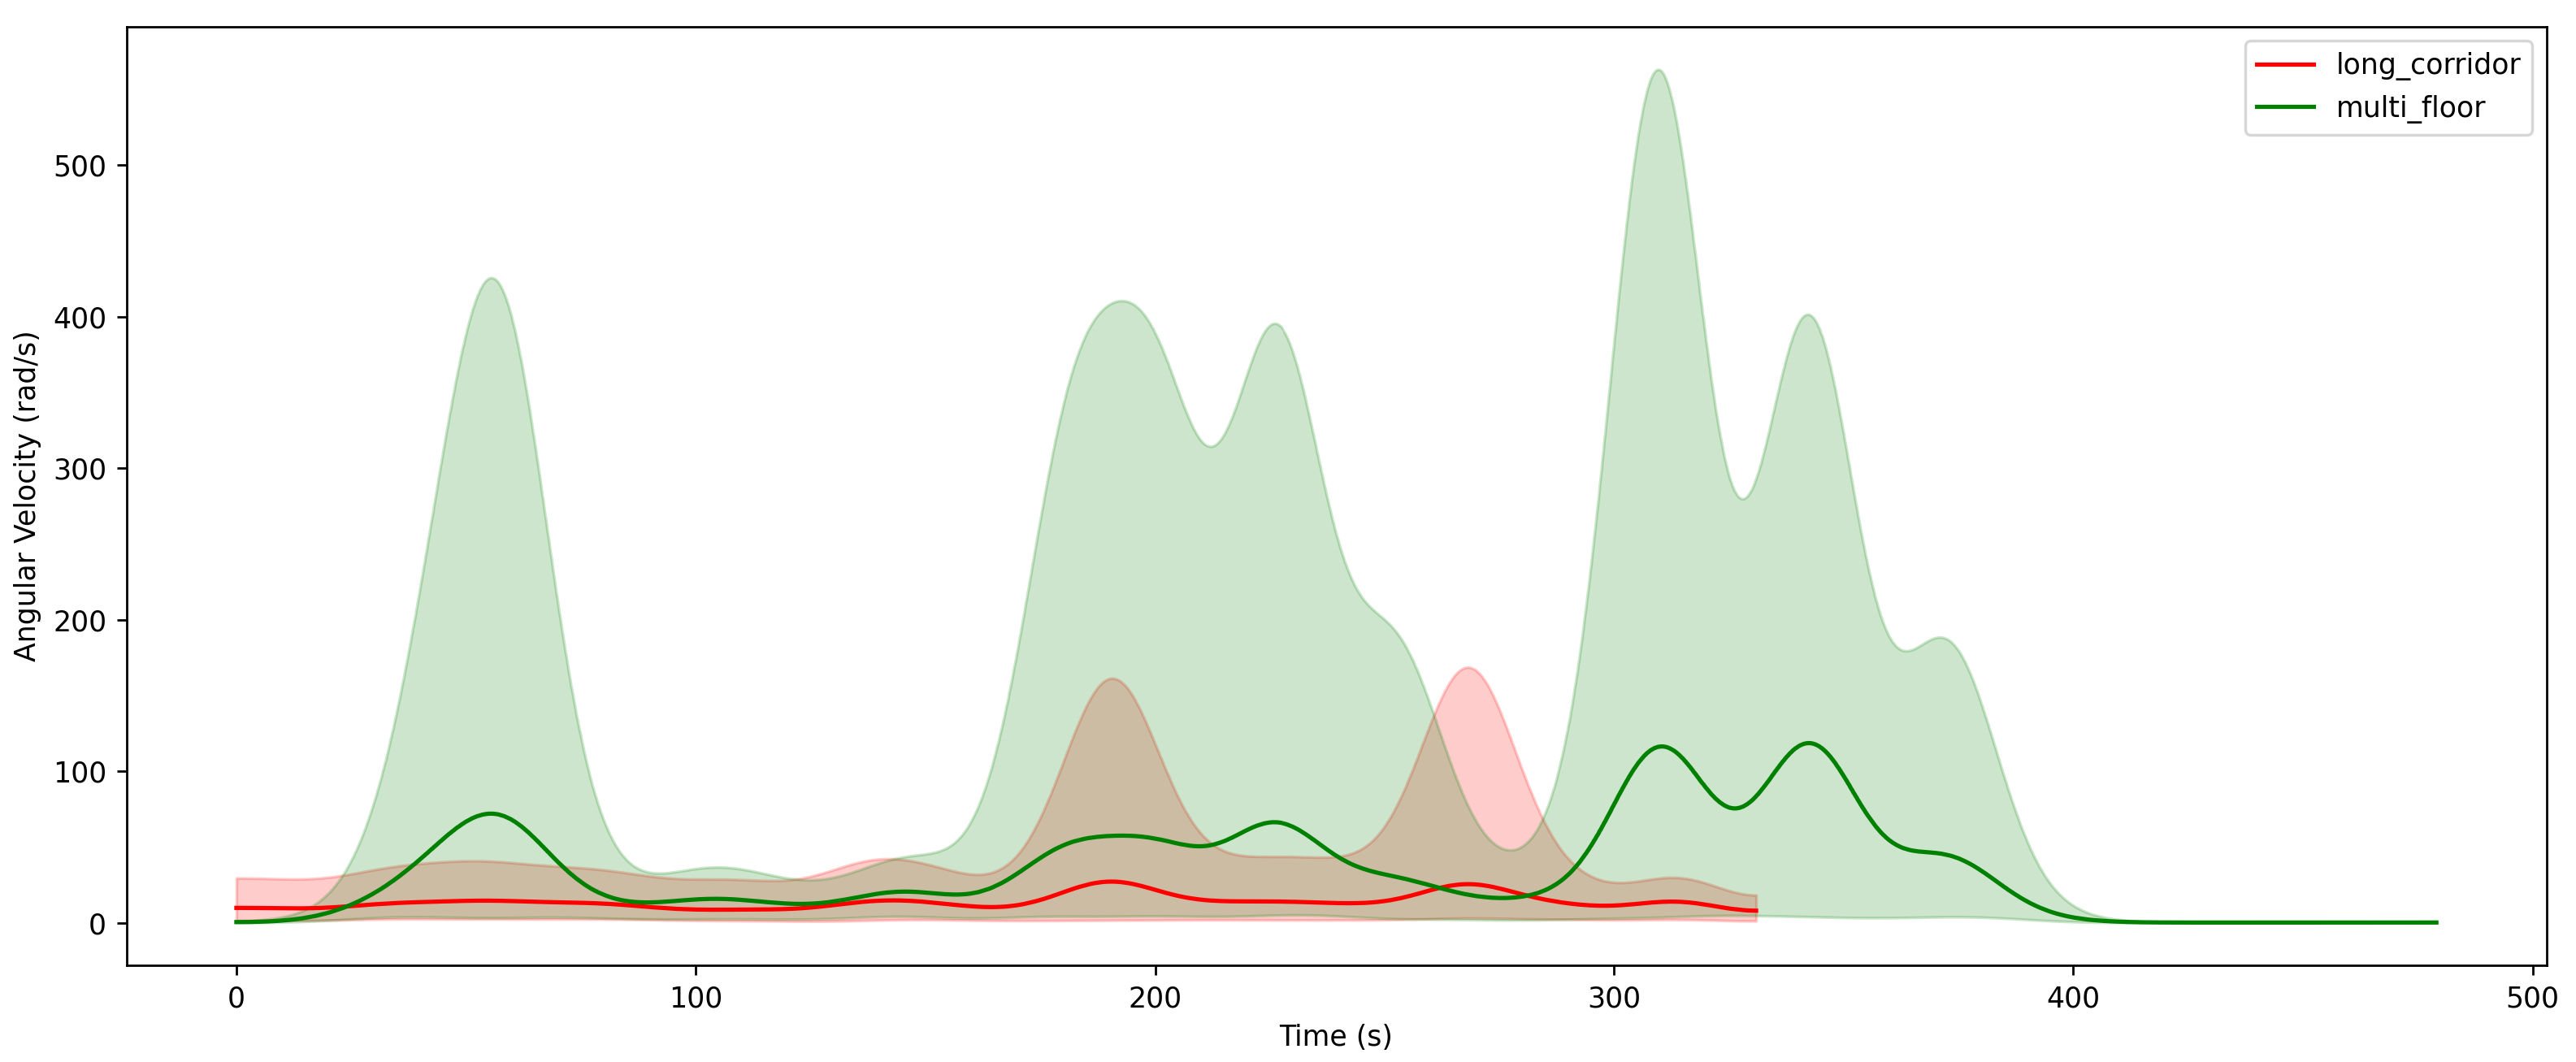
\includegraphics[width=0.9\textwidth,keepaspectratio]{figure/hawkins_angular.png}
%     \caption{The angular rate versus time graph for all runs collected in the Hawkins environment.}
%     \label{fig:hawkins_angular}
% \end{figure*}
% \begin{figure*}[ht!]
%     \centering
%     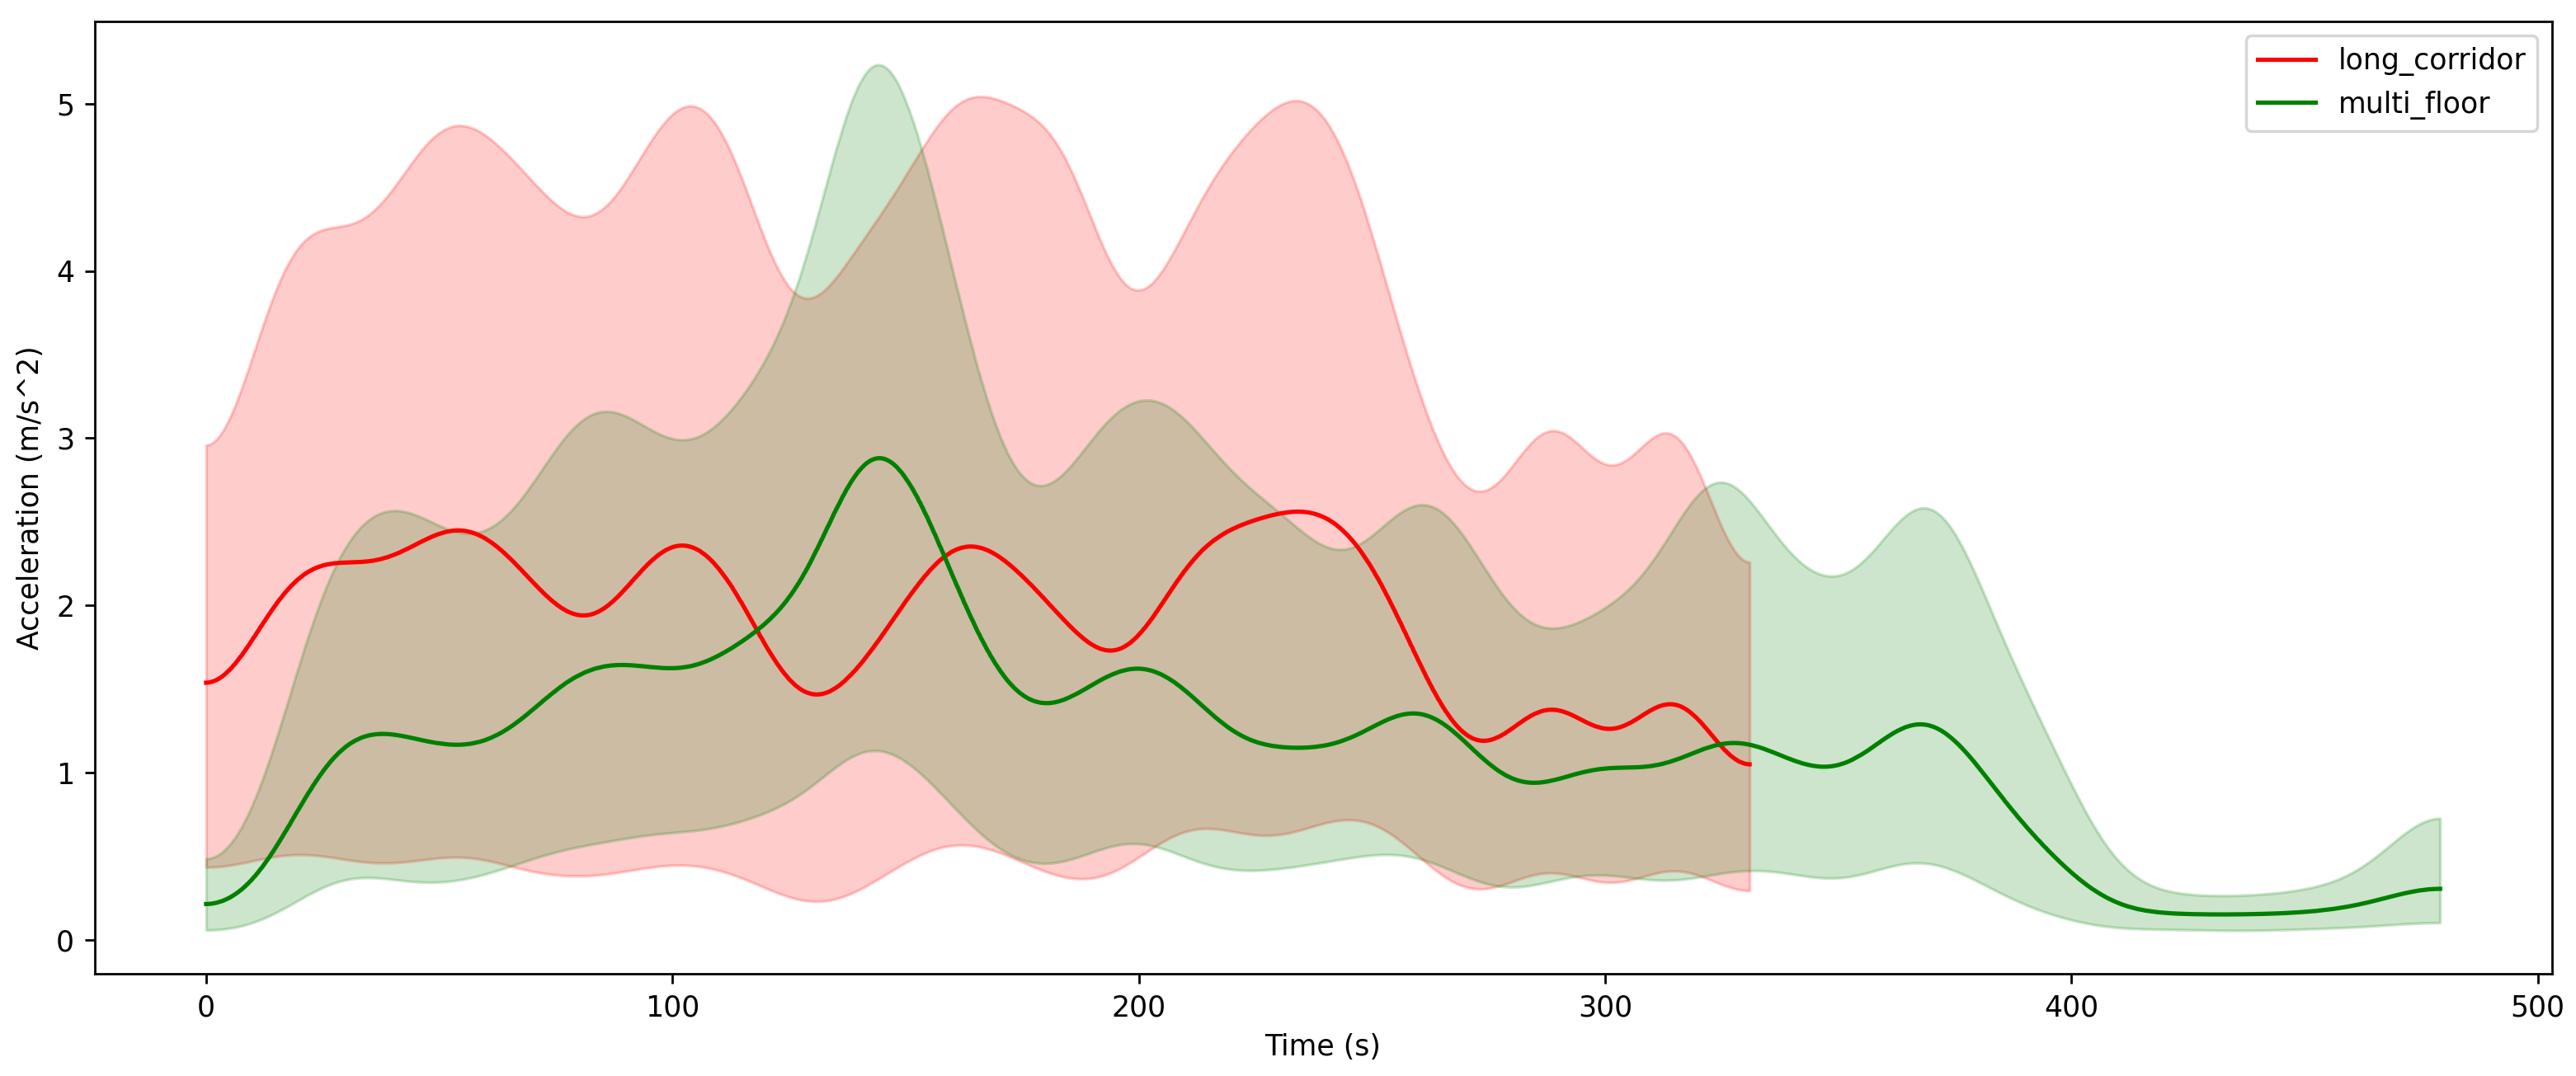
\includegraphics[width=0.9\textwidth,keepaspectratio]{figure/hawkins_accel.png}
%     \caption{The acceleration versus time graphs for all runs collected in the Hawkins environment.}
%     \label{fig:hawkins_accel}
% \end{figure*}
% \begin{figure*}[ht!]
%     \centering
%     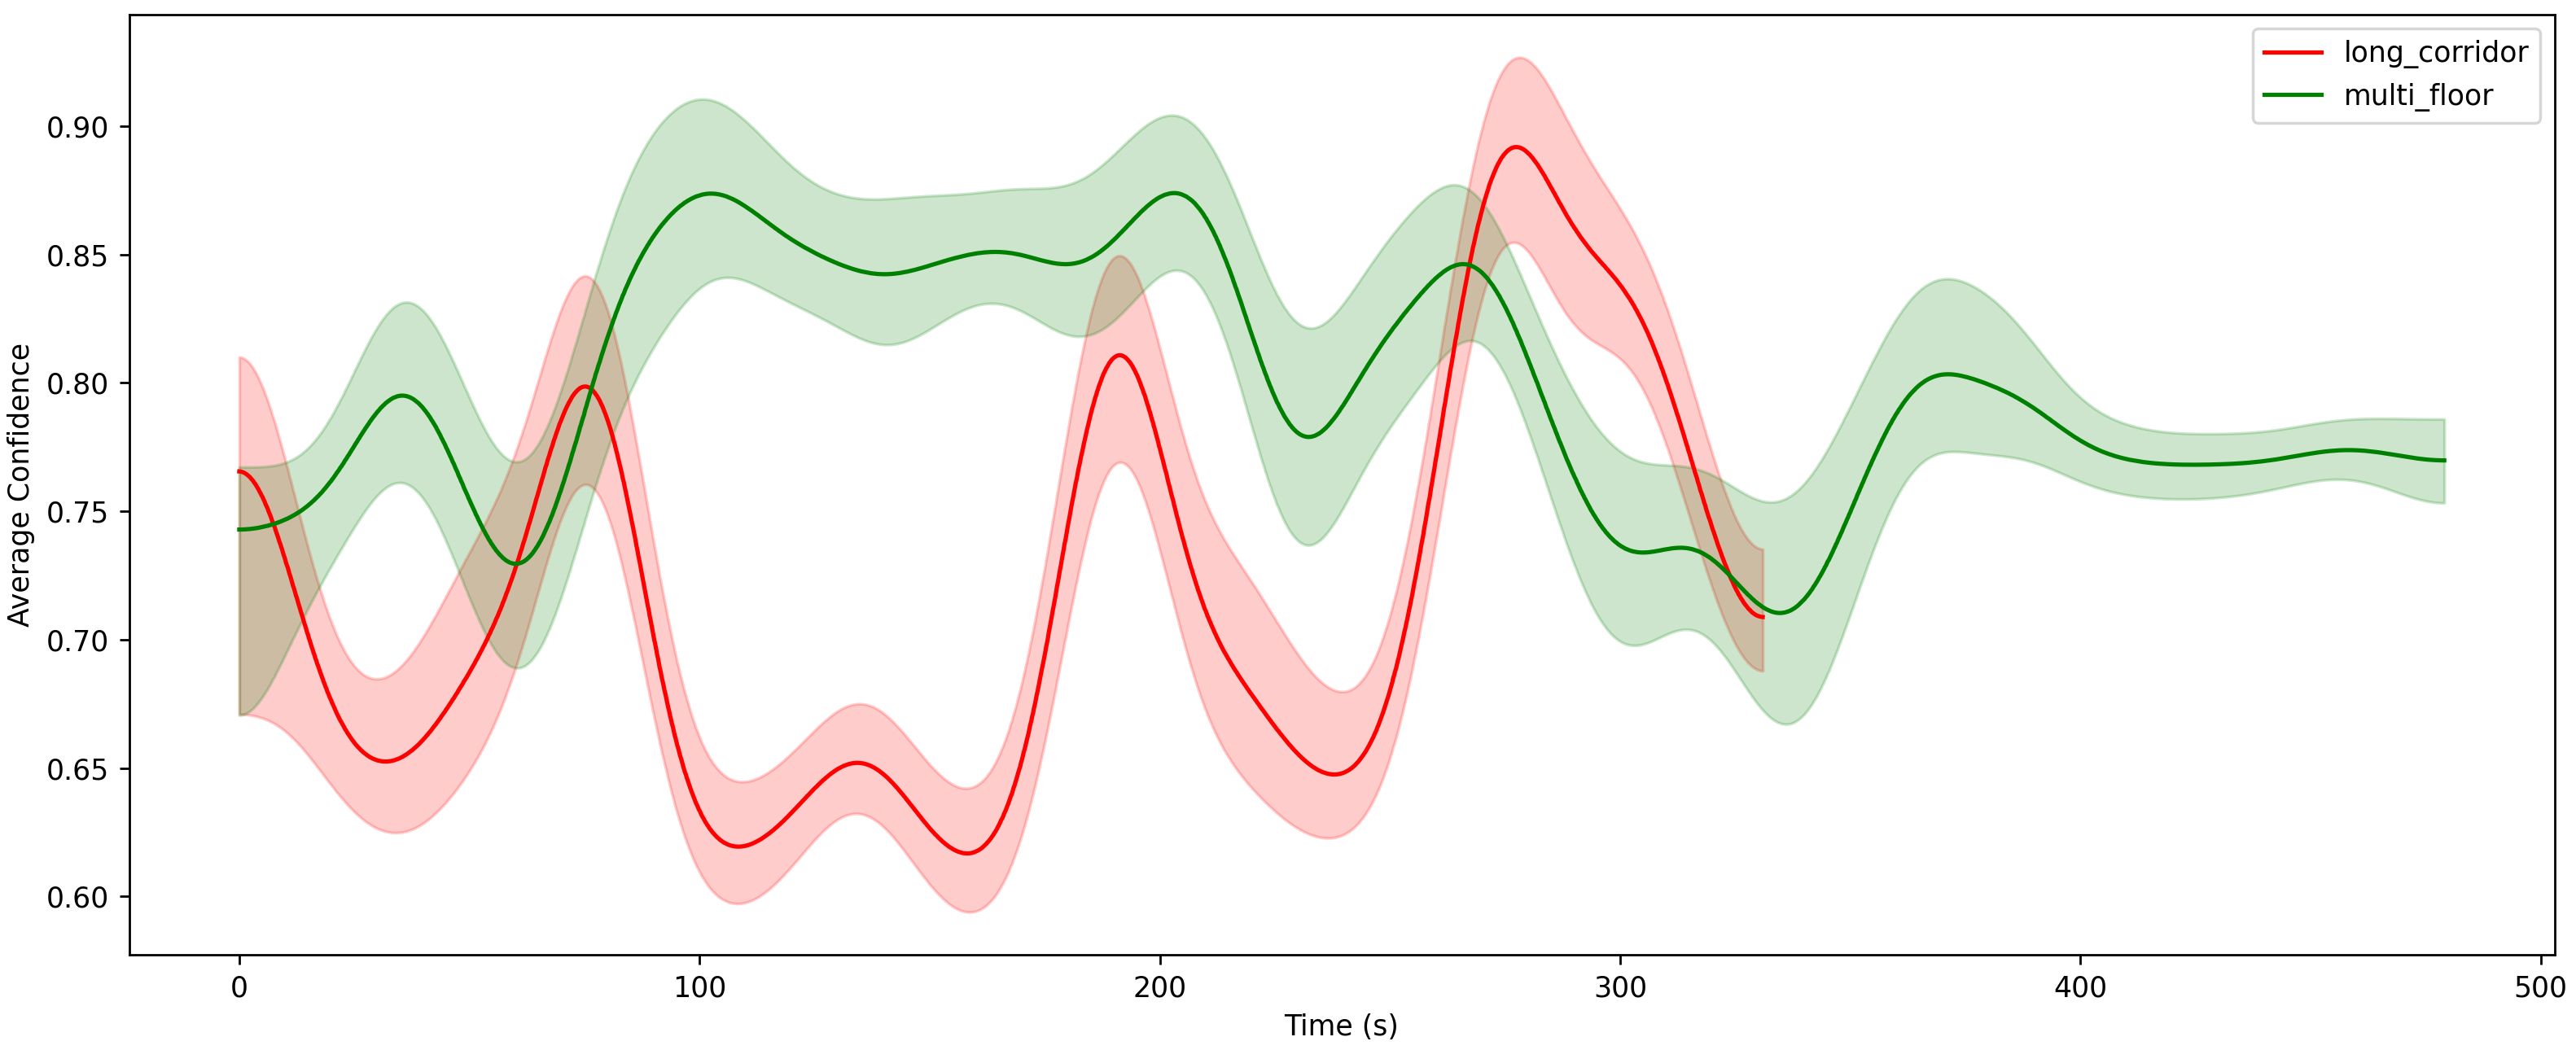
\includegraphics[width=0.9\textwidth,keepaspectratio]{figure/hawkins_confidence.png}
%     \caption{The confidence versus time graphs for all runs collected in the Hawkins environment.}
%     \label{fig:hawkins_confidence}
% \end{figure*}

% To help user download our datasets according to the difficulty, dataset evaluation is very neccessary. To achieve this, we adopt SuperOdometry to calculate vairous metrics to evalute the "difficulty". The statistics are including acceleration, angular velocity rate, and confidence value. The accleration and augular velocity is used to measure the motion pattern of this datasets and confidence value is provided by Super Odometry to evaluate the difficult of surrounding environments.  We plot the acceleration, angular velocity and confidence values for all the runs inclulding the Hawkins and Subt Challenge. For instance, figure \ref{fig:subt_accel} presents an evaluation of the $canary0921$ run in the SubT environment. The analysis reveals that the dataset from cannry drone is more challenging than other runs, as it displays a higher number of peaks and higher peak values on acceleration. Similarly, you can find more comparison on our other Fig.\ref{fig:subt_angular} Fig.\ref{fig:subt_confidence} Fig.\ref{fig:hawkins_accel} Fig.\ref{fig:hawkins_angular}.  

% % Analogous metrics are employed to evaluate the angular rate and translational uncertainty in the same context. This methodology provides a quantification of dataset complexity and a useful foundation for comparative analysis







% \begin{figure*}[ht!]
%     \centering
%     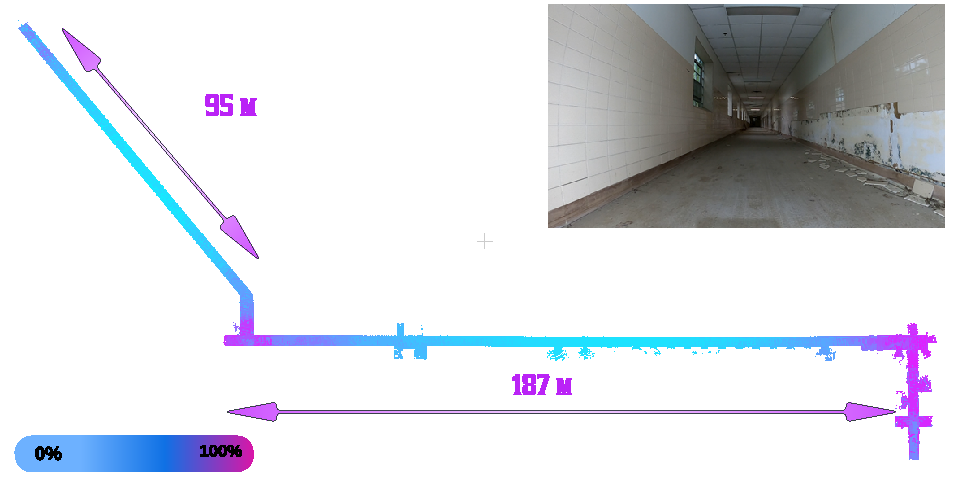
\includegraphics[width=0.9\textwidth,keepaspectratio]{figure/Long_Corridor_Uncertainty.pdf}
%     \caption{The Confidence Map From Super Odometry - It is important to note that in the confidence point cloud, areas that appear more blue indicate higher levels of uncertainty and risk for the robot during navigation. In the middle of long corridor area, It has the most blue areas. This is attributed to the limited constraints that the corridors provides in the X direction, which results in increased uncertainty in the mapping process}
%     \label{fig:uncertainty}
% \end{figure*}


% \section{Other GroundTruth 3D Models}

% In this section, we are delighted to showcase our comprehensive collection of Ground Truth 3D Models, as illustrated in Fig \ref{fig:Campus}, Fig\ref{fig:Hawkins1} and Fig\ref{fig:Hawkins2}. This collection features high-fidelity maps of various challenging environments, including long corridors, multiple floors, and poorly lit areas such as smoke rooms and darkness rooms. Moreover, we have included a ground truth model that encompasses a university campus, spanning both indoor and outdoor areas. It's worth noting that all the ground truth models were obtained using a FARO scanner, ensuring accuracy within 2 cm.






% \begin{figure*}[bh!]
%   \centering
%   \begin{subfigure}[b]{0.48\textwidth}
%     \centering
%     \includegraphics[width=\textwidth]{figure/ground_truth_hawkins.png}
%     \caption{The Ground Truth Model from Indoor to Outdoor}
%     \label{fig:dc1}
%   \end{subfigure}
%   \hfill
%   \begin{subfigure}[b]{0.48\textwidth}
%     \centering
%     \includegraphics[width=\textwidth]{figure/ground_truth_building_4_side.png}
%     \caption{The Ground Truth Model for Multiple Floor}
%     \label{fig:dc2}
%       \end{subfigure}
%   \caption{The Ground Truth Model in Hawkins Environments}
%     \label{fig:Hawkins1}
% \end{figure*}


% \begin{figure*}[bh!]
%   \centering
%   \begin{subfigure}[b]{0.48\textwidth}
%     \centering
%     \includegraphics[width=\textwidth]{figure/hawkins_big_loop.png}
%     \caption{The Ground Truth Model for Long Corridor Environments}
%     \label{fig:dc3}
%   \end{subfigure}
%   \hfill
%   \begin{subfigure}[b]{0.48\textwidth}
%     \centering
%     \includegraphics[width=\textwidth]{figure/top_down_building_4.png}
%     \caption{The Ground Truth Model for Multiple  Floor }
%     \label{fig:dc4}
%       \end{subfigure}
%  \caption{The Ground Truth Model in Hawkins Environments}
%   \label{fig:Hawkins2}
% \end{figure*}

% \begin{figure*}[bh!]
%   \centering
%   \begin{subfigure}[b]{0.48\textwidth}
%     \centering
%     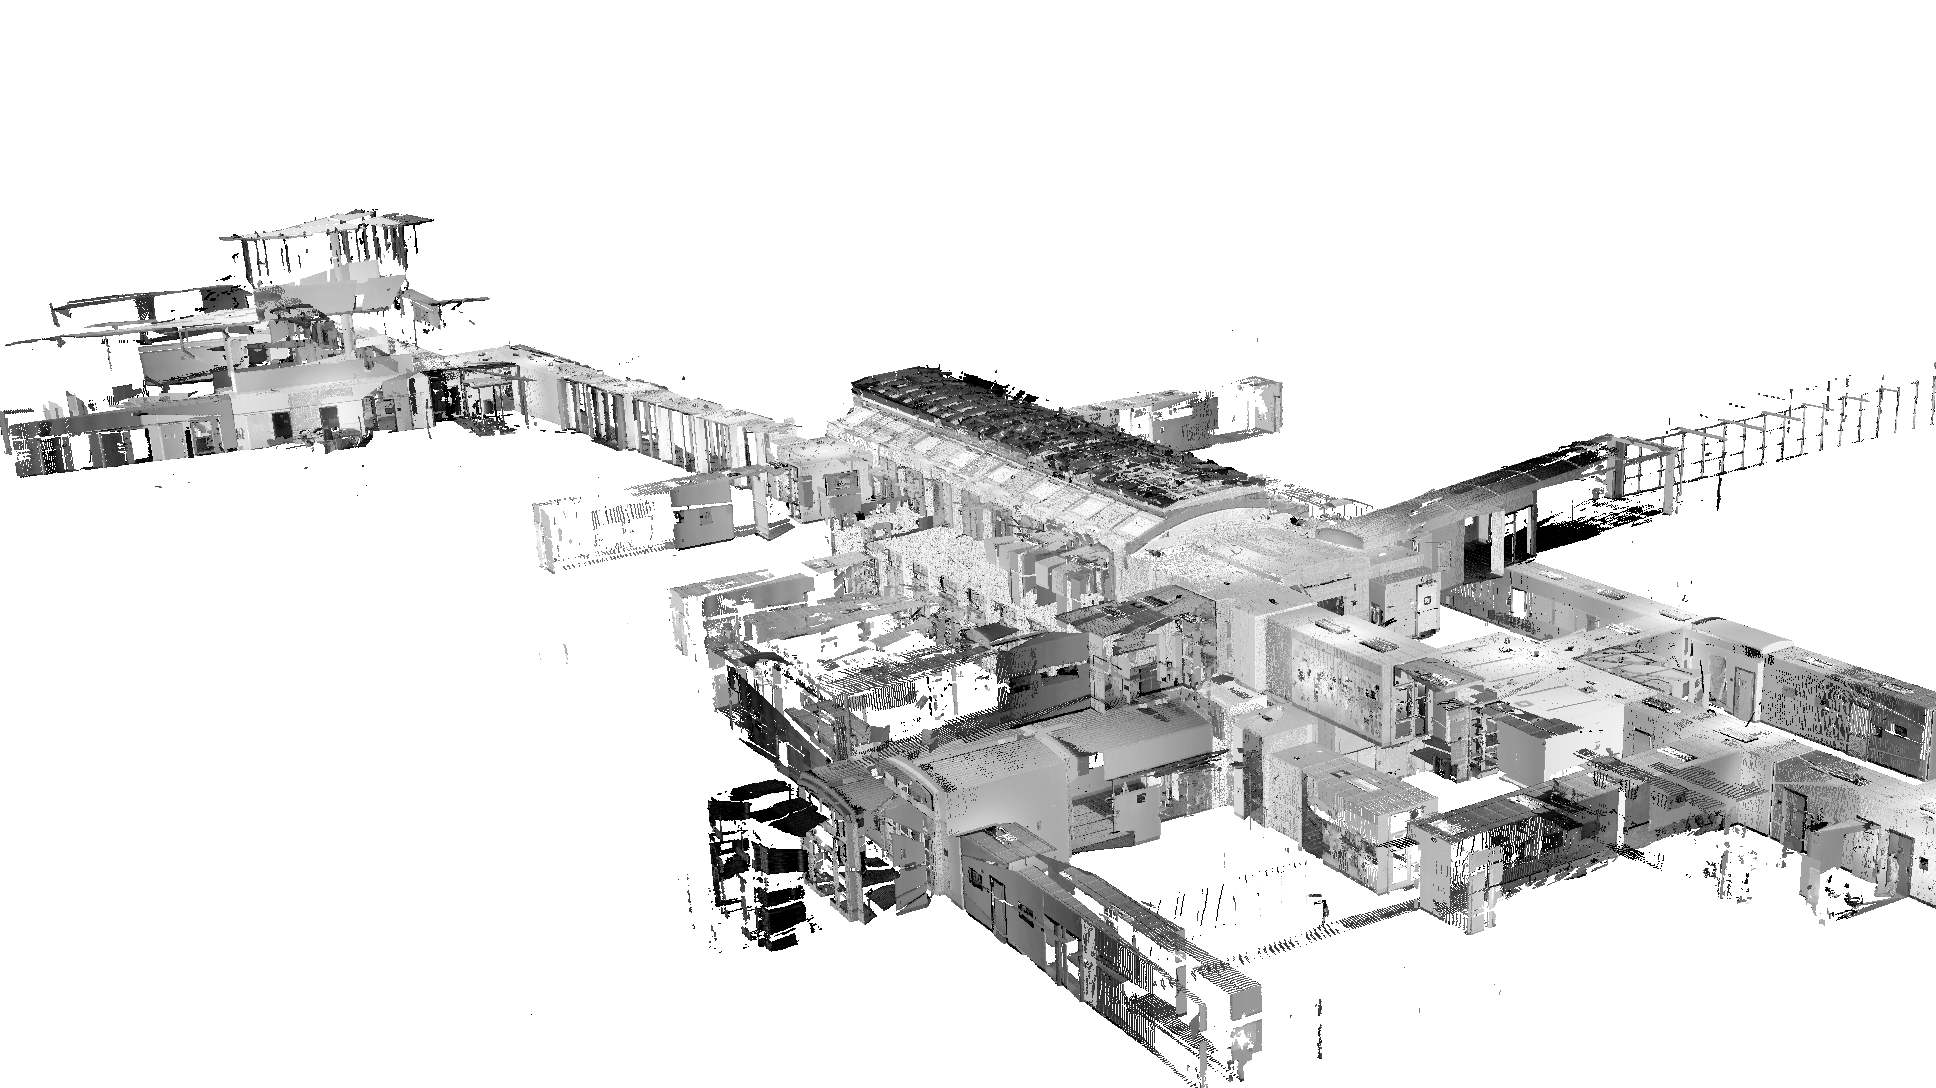
\includegraphics[width=\textwidth]{figure/nsh_internal.png}
%     \caption{The Ground Truth Model in University Campus for Indoor Environments}
%     \label{fig:dc5}
%   \end{subfigure}
%   \hfill
%   \begin{subfigure}[b]{0.48\textwidth}
%     \centering
%     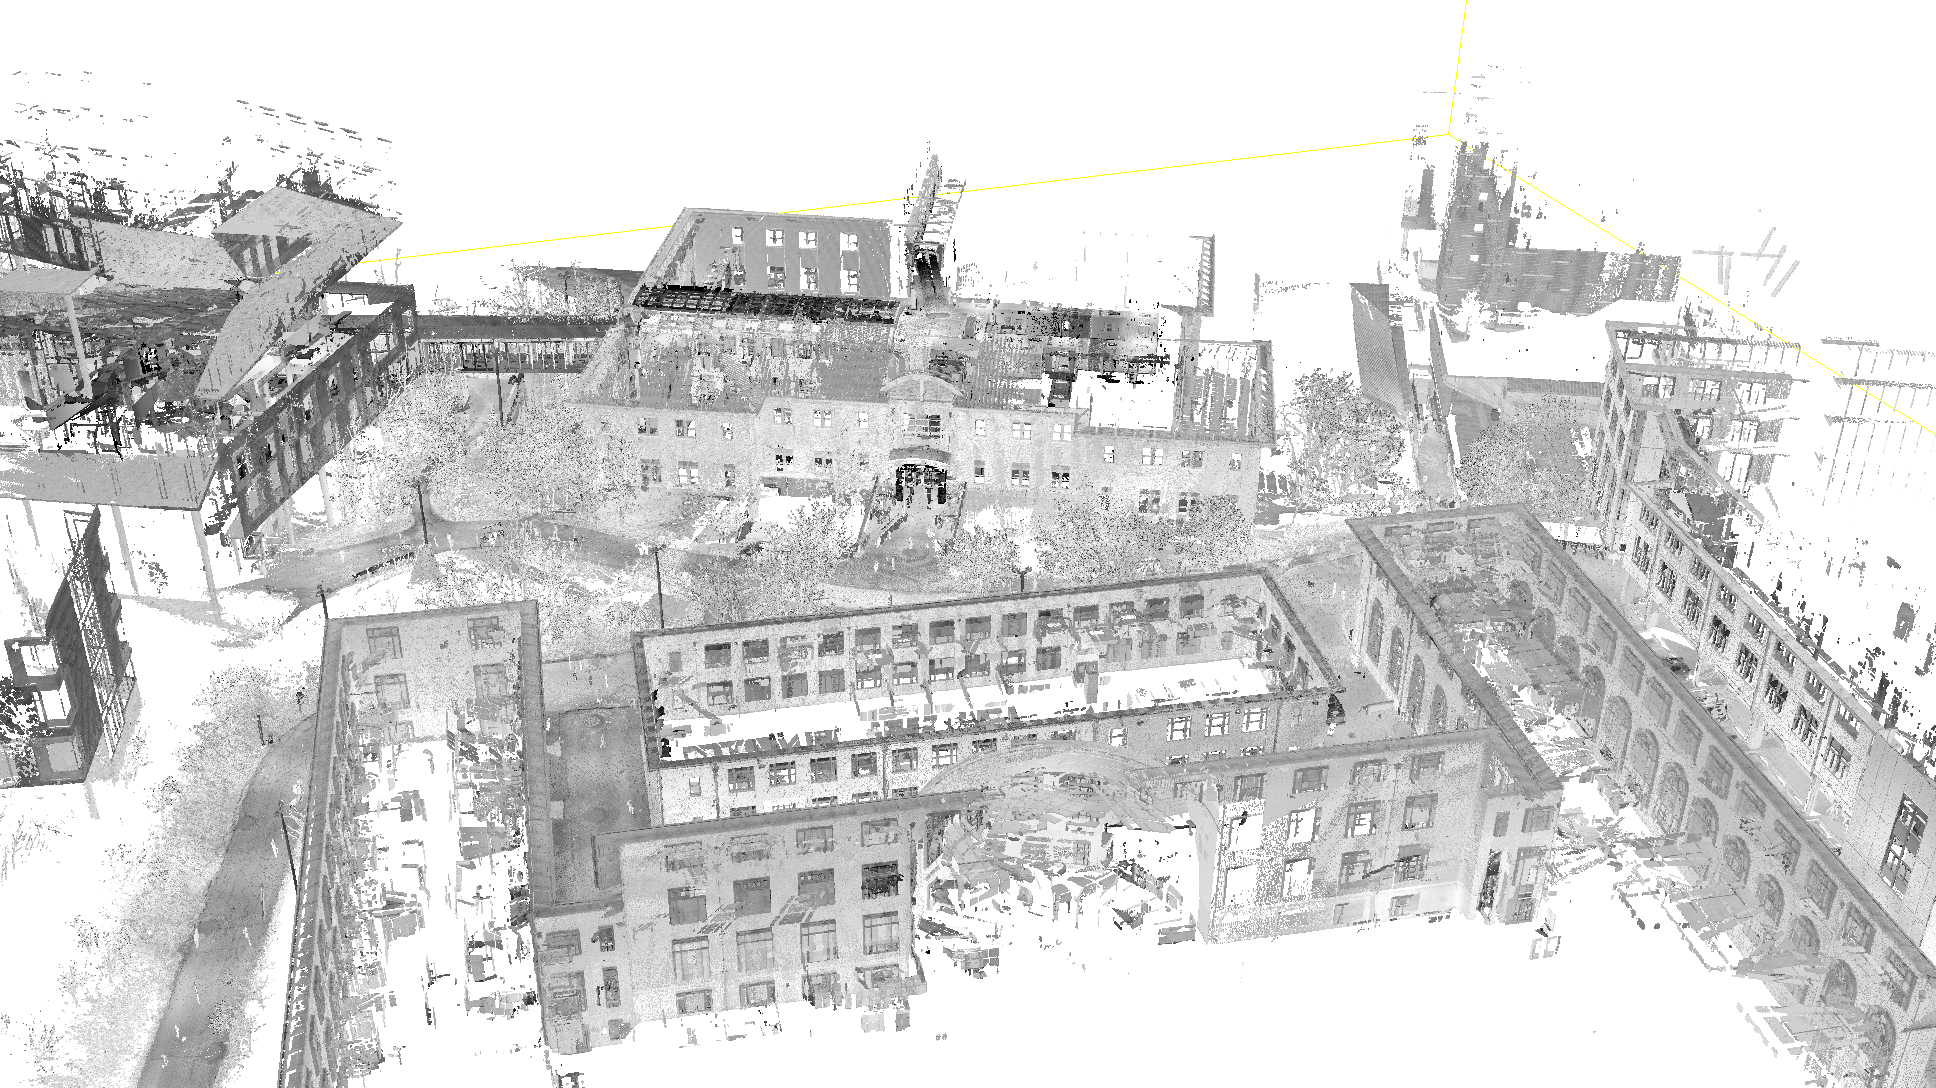
\includegraphics[width=\textwidth]{figure/nsh_overall.png}
%     \caption{The Ground Truth Model in University Campus for Outdoor Environments}
%     \label{fig:dc6}
%       \end{subfigure}
% \caption{The Ground Truth Model in University Campus}
%   \label{fig:Campus}
% \end{figure*}




% % \begin{table*}\footnotesize
% % \caption{Summary of the experiment sequences.}
% % \begin{tabular}{c||c|c|c|c|c|c|c|c}
% % \toprule
% % Sequence & Difficulty level & In-/outdoor & Smoke                     & Low illumination          & Overexposure              & Long corridor             & Motion pattern   & Trajectory length \\ \midrule
% % run1     & easy             & indoor      & \CheckmarkBold & \XSolidBrush    & \XSolidBrush    & \XSolidBrush    & mild handheld    & short             \\ \hline
% % run2     & easy             & indoor      & \CheckmarkBold & \XSolidBrush    & \XSolidBrush    & \XSolidBrush    & mild handheld    & short             \\ \hline
% % run3     & middle           & indoor      & \CheckmarkBold & \XSolidBrush    & \XSolidBrush    & \XSolidBrush    & mild handheld    & long              \\ \hline
% % run4     & middle           & outdoor     & \XSolidBrush    & \CheckmarkBold & \XSolidBrush    & \XSolidBrush    & legged robot             & middle            \\ \hline
% % run5     & difficult        & indoor      & \XSolidBrush    & \XSolidBrush    & \CheckmarkBold & \XSolidBrush    & legged robot             & middle            \\ \hline
% % run6     & difficult        & indoor      & \CheckmarkBold & \XSolidBrush    & \XSolidBrush    & \XSolidBrush    & drastic handheld & long              \\ \hline
% % run7     & magistrale       & mixed       & \CheckmarkBold & \CheckmarkBold & \XSolidBrush    & \CheckmarkBold & drastic handheld & long              \\ 
% % \bottomrule

% % \end{tabular}
% % \label{trajSummary}

% % \end{table*}









% % \section{Limitations} \label{sec:limitations}
% % This section will give further details and explanations, which were not mentioned in the main paper due to the constrained space, regarding the limitations of the proposed datasets.




\end{document}




